This section presents the verification and performance results of the presented FEM-BEM coupling schemes, for molecules modeled as cavities with constant and varying permittivity.
With a constant permittivity inside the molecule, we tested convergence against an analytical expression of the solvation energy of a sphere \cite{Kirkwood1934}, and then compared a more realistic geometry (arginine) with a purely BEM implementation.
We also considered a Gaussian-varying permittivity\cite{grant2001smooth,li2013dielectric} inside the molecular cavity of arginine, and used APBS \cite{BakerETal2001} to verify our results.
The final tests show the scaling of the FEM-BEM coupling, as the molecule size grows. 

All runs were done on XX computer with YY specifications. 

\section*{\sffamily \Large Software environment}

For the finite element computations, we use the software package FEniCSx while for the boundary element computations we use Bempp-cl together with Exafmm-t. FEniCSx is the successor of the widely used FEniCS finite element library.
It provides a convenient Python interface, in which problems are described using UFL (Unified Form Language), a convenient domain-specific language specifically designed for finite element discretisations of partial differential equations. During assembly the UFL description is transformed into efficient low-level C++ code and just-in-time compiled. Bempp-cl is a Python package that uses low-level OpenCL kernels written in C99 to provide optimised assembly routines. The built-in dense assembly routines are highly efficient for moderate discretisation sizes up to a few ten thousand elements.

For very large grid sizes the user can enable FMM assembly which internally is handled in Bempp-cl through an interface to the Exafmm-t FMM library. For $N$ surface elements this reduces the memory and computational complexity from $\mathcal{O}(N^2)$ in the dense assembly case to $\mathcal{O}(N)$ in the FMM case, making large boundary element problems tractable on standard workstations.

To couple FEniCSx with Bempp-cl we load a volume mesh with FEniCSx. We then export the corresponding boundary mesh into Bempp-cl and assemble the boundary spaces there. Bempp-cl provides numerical trace operators that can translate from the degree of freedom (dof) representation in FEniCSx to the dof representation in Bempp-cl. The corresponding translation work is handled opaquely and the user only needs to deal with high-level interfaces of FEniCSx operators, Bempp-cl operators, and trace operators. FMM assembly fits automatically into this framework and can be enabled or disabled as simple configuration option.

Docker images containing FEniCSx, Bempp-cl, and Exafmm-t are publicly available (PROVIDE LINK), and all codes used in this sections are simple Jupyter Notebooks that can be reproducibly executed in this provided Docker image.

\section*{\sffamily \Large Results with constant permitivitty}

In implicit-solvent models, the molecule is usually considered as a region with constant permittivity, in this case, with $\epsilon_1=2$.
In the solvent region, we used the permittivity of water ($\epsilon_2$=80) and an inverse of the Debye length of $\kappa=0.125$ \AA$^{-1}$.
As in these cases there is an analytical solution for $\phi_c$ in Eq. \eqref{eq:phic}, we compute $\phi_r$ with Eq. \eqref{eq:phi_reac} in both BEM-BEM and FEM-BEM coupling approaches. Then, for FEM-BEM, the integral over $\Gamma$ in Eq. \eqref{eq:phi_reac} corresponds to the trace of the solution vector.

\subsection*{\sffamily \large Convergence of a spherical cavity}

The Kirkwood sphere \cite{Kirkwood1934} is a standard benchmark test for the Poisson-Boltzmann equation in molecular electrostatics. 
In this case, we considered a spherical cavity of radius $R=2$ \AA, with three charges ($q_1$=1, $q_2$=1, and $q_3$=0.75) placed at $\mathbf{x}_1=(1,0,0)$, $\mathbf{x}_2=(0.7,0.7,0)$, and $\mathbf{x}_3=(-0.5,-0.5,0)$.
Figure \ref{fig:error_sphere} shows the error convergence of the FEM-BEM approaches, and a reference BEM implementation, to the analytical solution ($\Delta G_{solv}= -336.0396$ kcal/mol). 
In these runs, the FEM mesh was generated using GMSH~\cite{geuzaine2009gmsh} 
%Bempp (check?) from a surface discretization 
with %1, 2, 4, and 8 
2, 6, 21 and 83 vertices per \AA$^2$ on the SES, the surface mesh of this volume one was also used for the BEM runs. 
%For the hybrid FEM-BEM coupling approach, we used $\tau$=5.
The error in Figure \ref{fig:error_sphere} decays linearly with the surface area, which agrees with the expected convergence for P1 elements, indicating a correct implementation of the numerical scheme. 
%We can see that the purely BEM implementation outperforms (or not?) FEM-BEM coupling in terms of accuracy for equivalent meshes, and also that the hybrid approach does not (or does?) influence accuracy. 

\begin{figure}
  \centering
  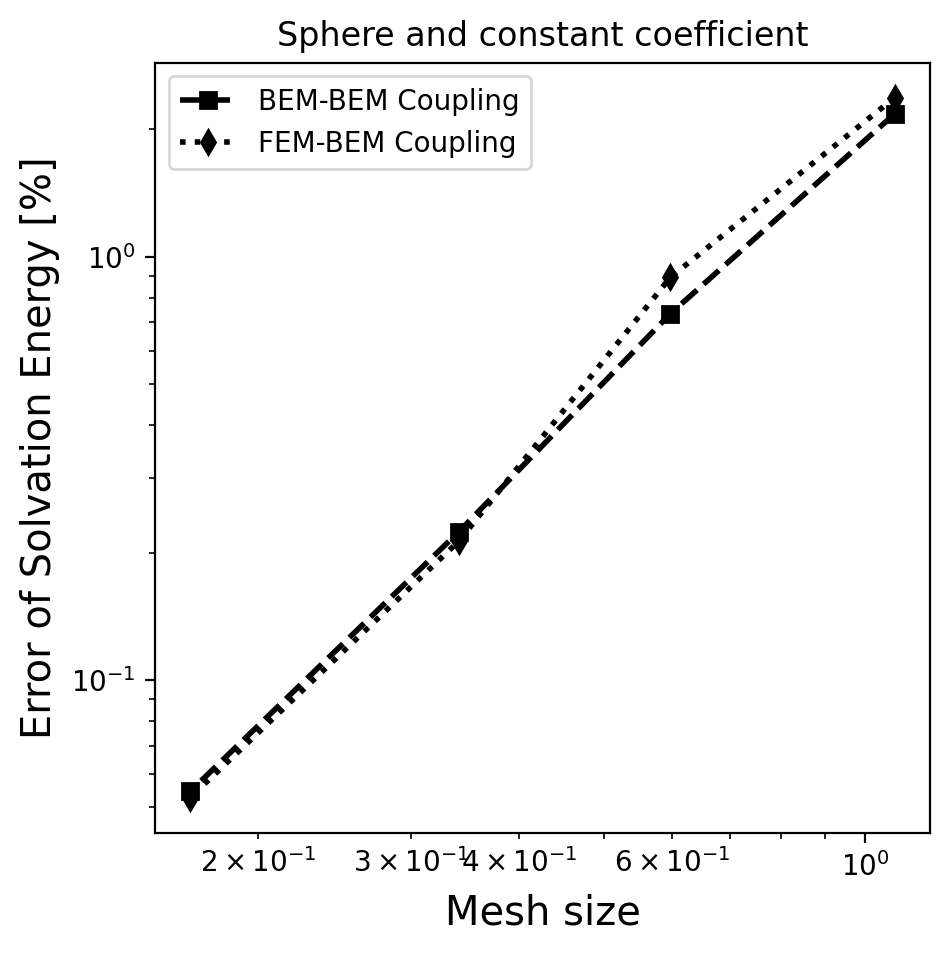
\includegraphics[width=0.6\linewidth]{DolfinX_Sphere_const_coeff_error.png}
  \caption{Error for the Kirkwood sphere.}
  \label{fig:error_sphere}
\end{figure}

\subsection*{\sffamily \large Performance with arginine}

As a more realistic test, we assessed the performance of the FEM-BEM coupling technique against a purely BEM implementation for arginine (the structure of arginine taken from the protein data bank \cite{bank}). 
We generated surface meshes containing W, X, Y, and Z vertices per \AA$^2$ with Nanoshaper.~\cite{decherchi2013general}
These meshes were inputs to our purely BEM solver, and to create the FEM mesh with pyGAMer,~\cite{lee2020open} which invoked \texttt{tetgen} [citation] with the string \texttt{abcd}.

The solvation energy computed with the two schemes is presented by Figure \ref{fig:arg_constant_energy}, which, as expected, converges to a similar answer as the mesh is refined.
Then, Figure \ref{fig:arg2_constant_time_iter} compares the iteration count and time-to-solution. The left plot shows that using only BEM outperforms the coupled FEM-BEM approach in terms of iterations count. However, if we look at the total time that solvers take to obtain the solution, we can see the advantage of using the FEM-BEM coupling. The higher computational cost is caused by the need of using a hypersingular operator in the BEM formulation.


\begin{figure}
\centering
   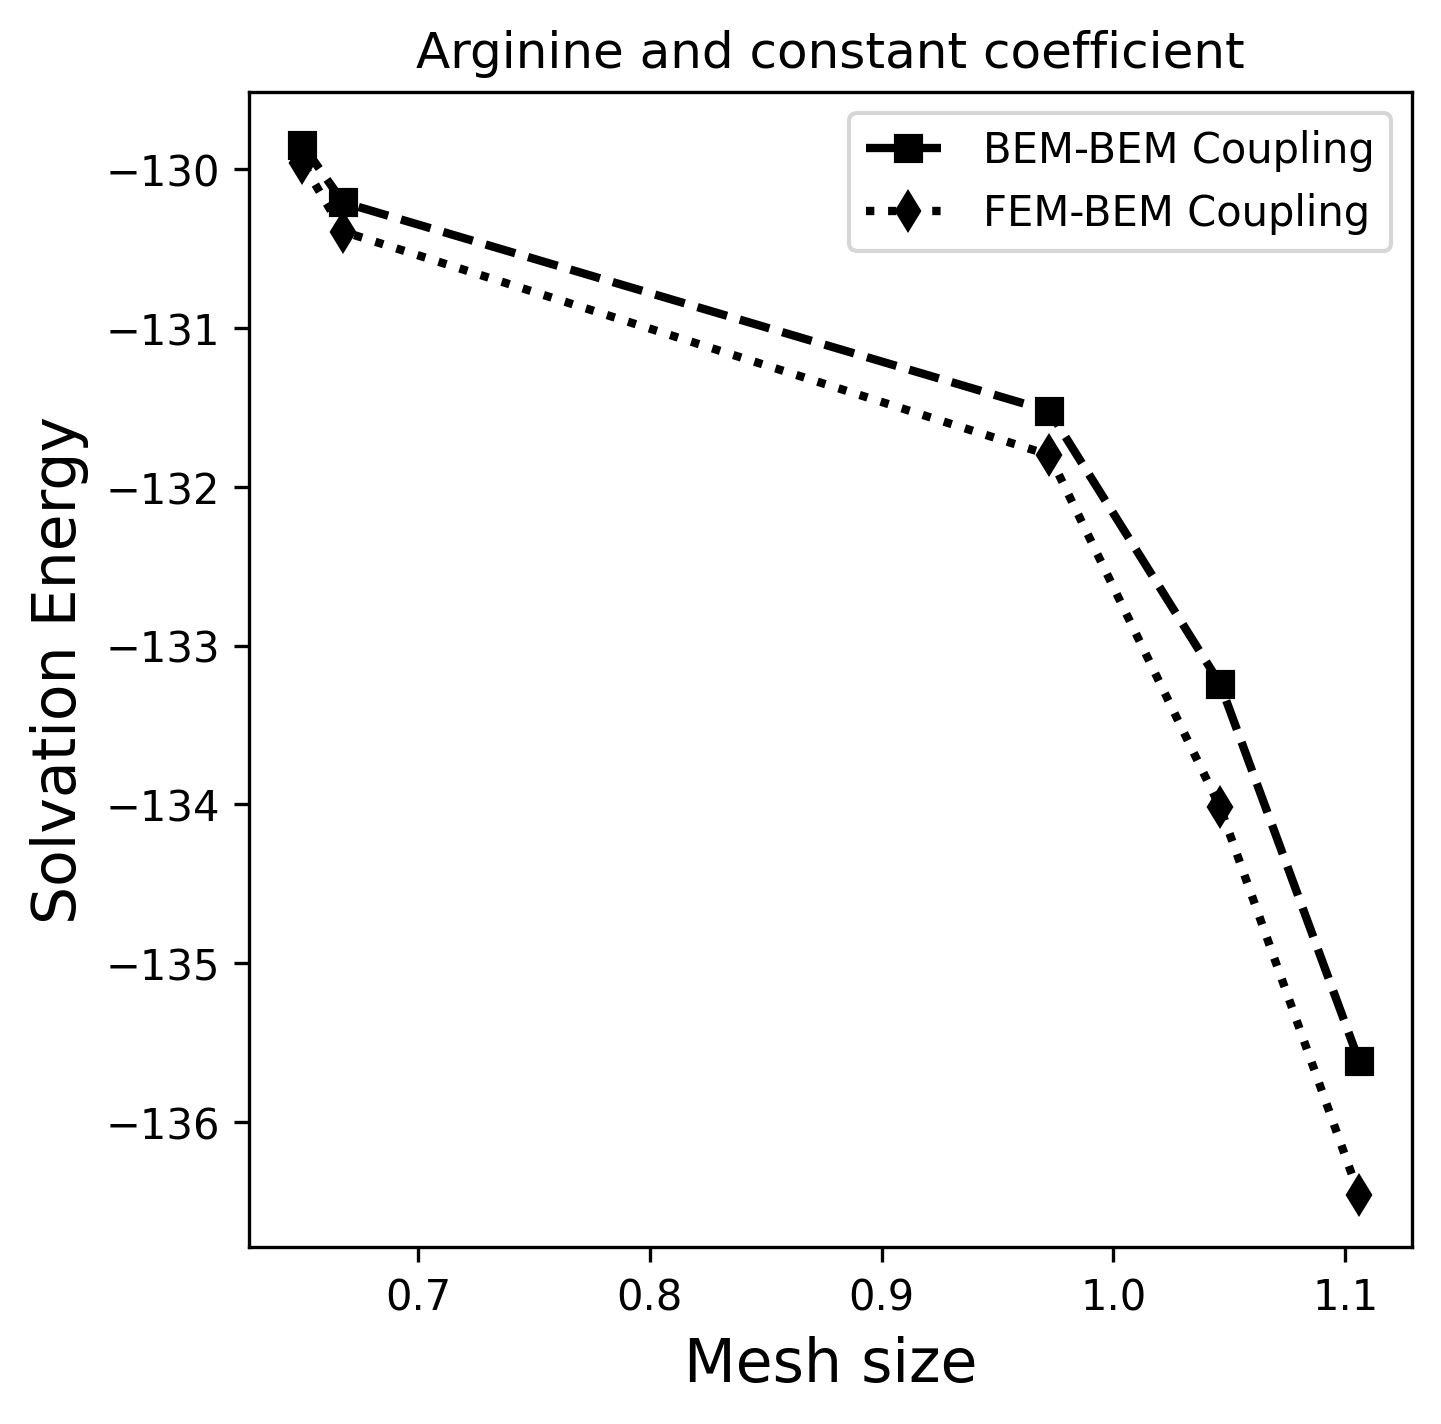
\includegraphics[width=0.47\linewidth]{DolfinX_Arginine2_const_coeff_error.png}
%   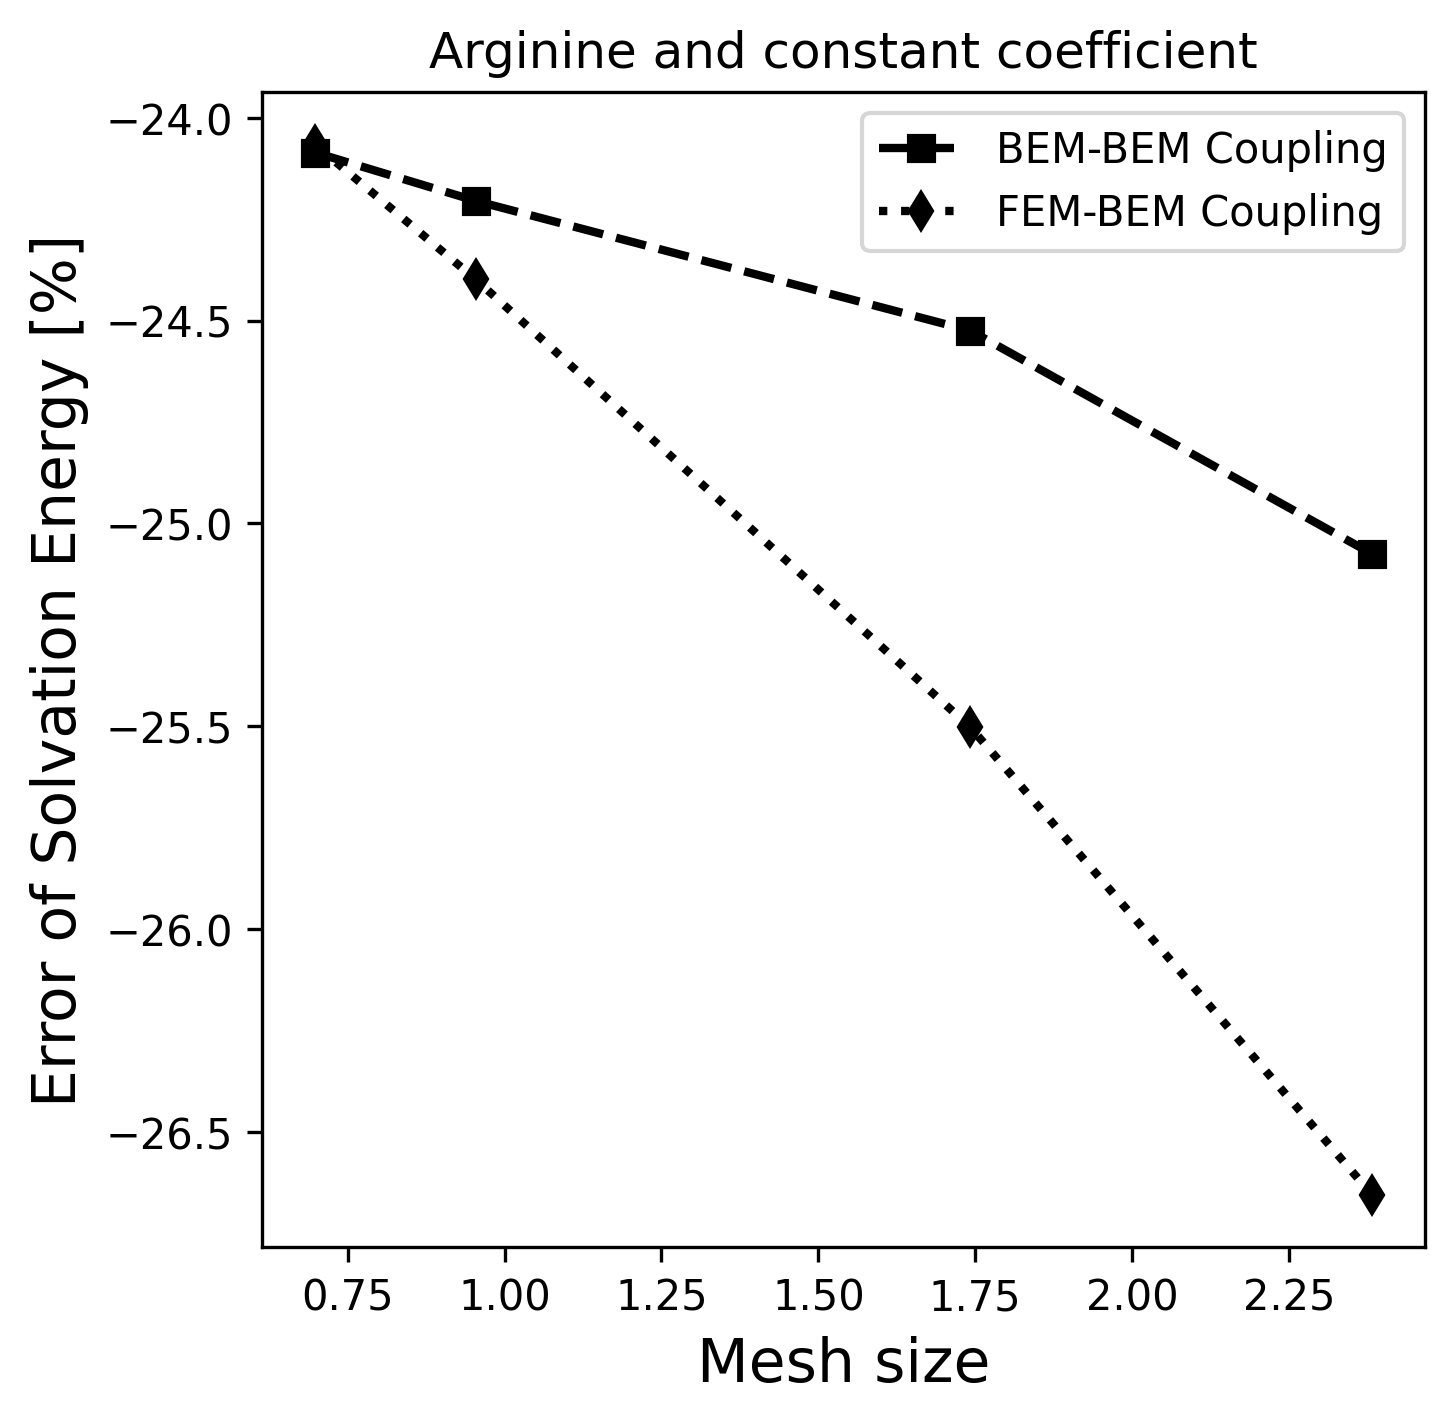
\includegraphics[width=0.47\linewidth]{DolfinX_Arginine_const_coeff_error_11.png}
\caption{Solvation energy for arginine with a constant permittivity. %(left - Arginine2 and right - Arginine)
%maybe we could also add a "error" wrt extrapolation, or a plot with energy for each mesh?
}
\label{fig:arg_constant_energy}
\end{figure}

\begin{figure}
\centering
   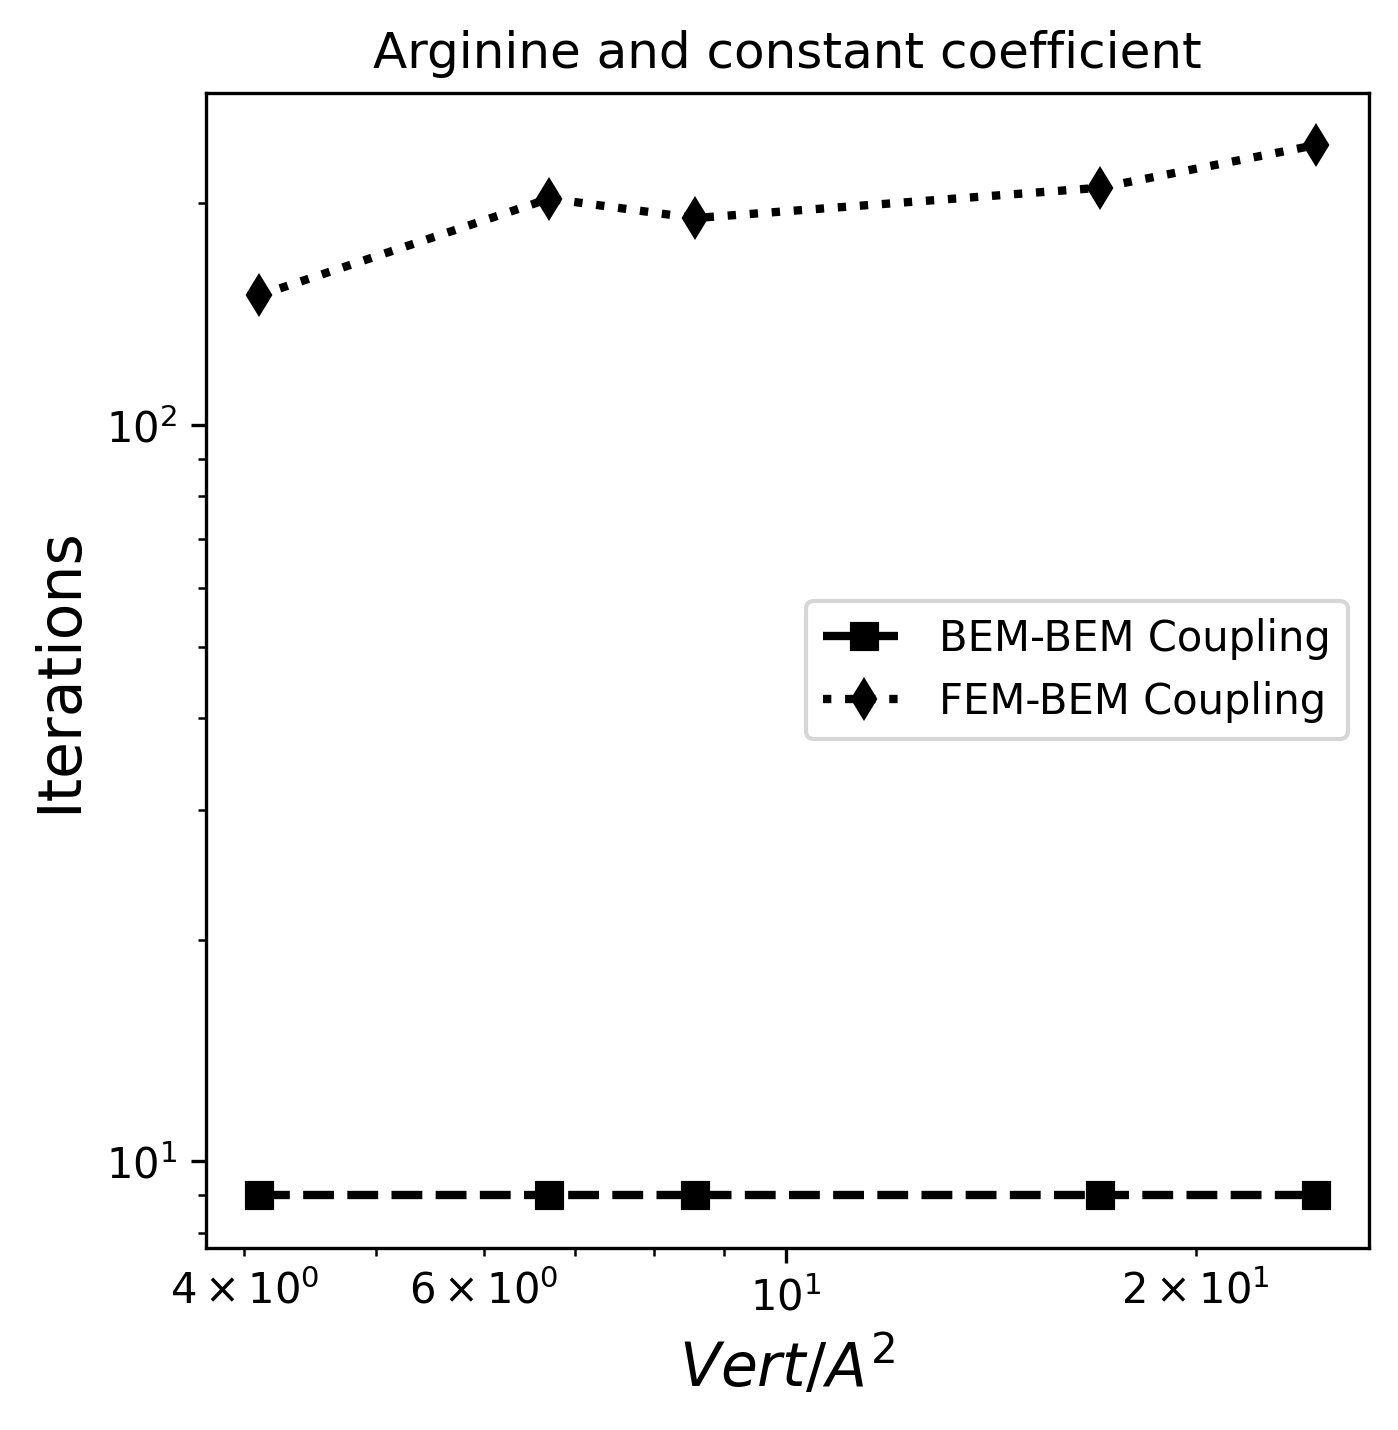
\includegraphics[width=0.45\linewidth]{DolfinX_Arginine2_const_coeff_iter.png}
%  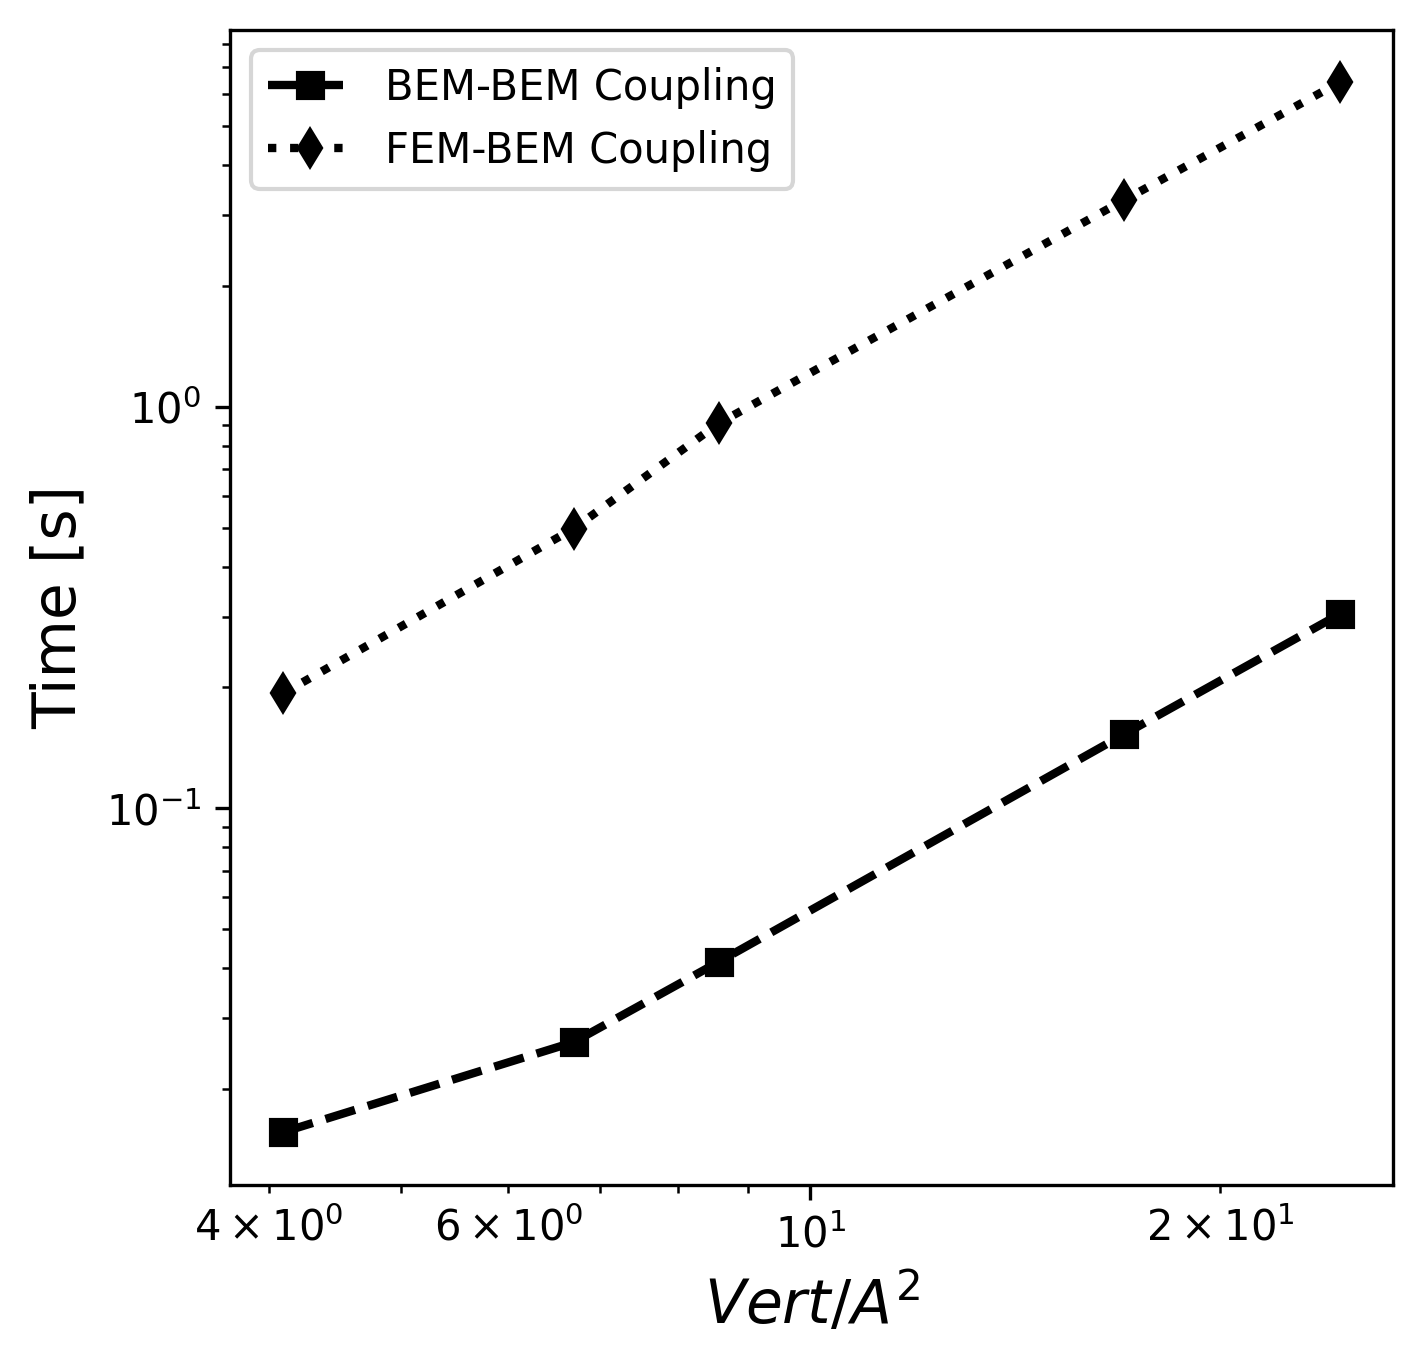
\includegraphics[width=0.45\linewidth]{DolfinX_Arginine2_const_coeff_time.png}
%  \includegraphics[width=0.45\linewidth]{DolfinX_Arginine2_const_coeff_setup_time.png}
  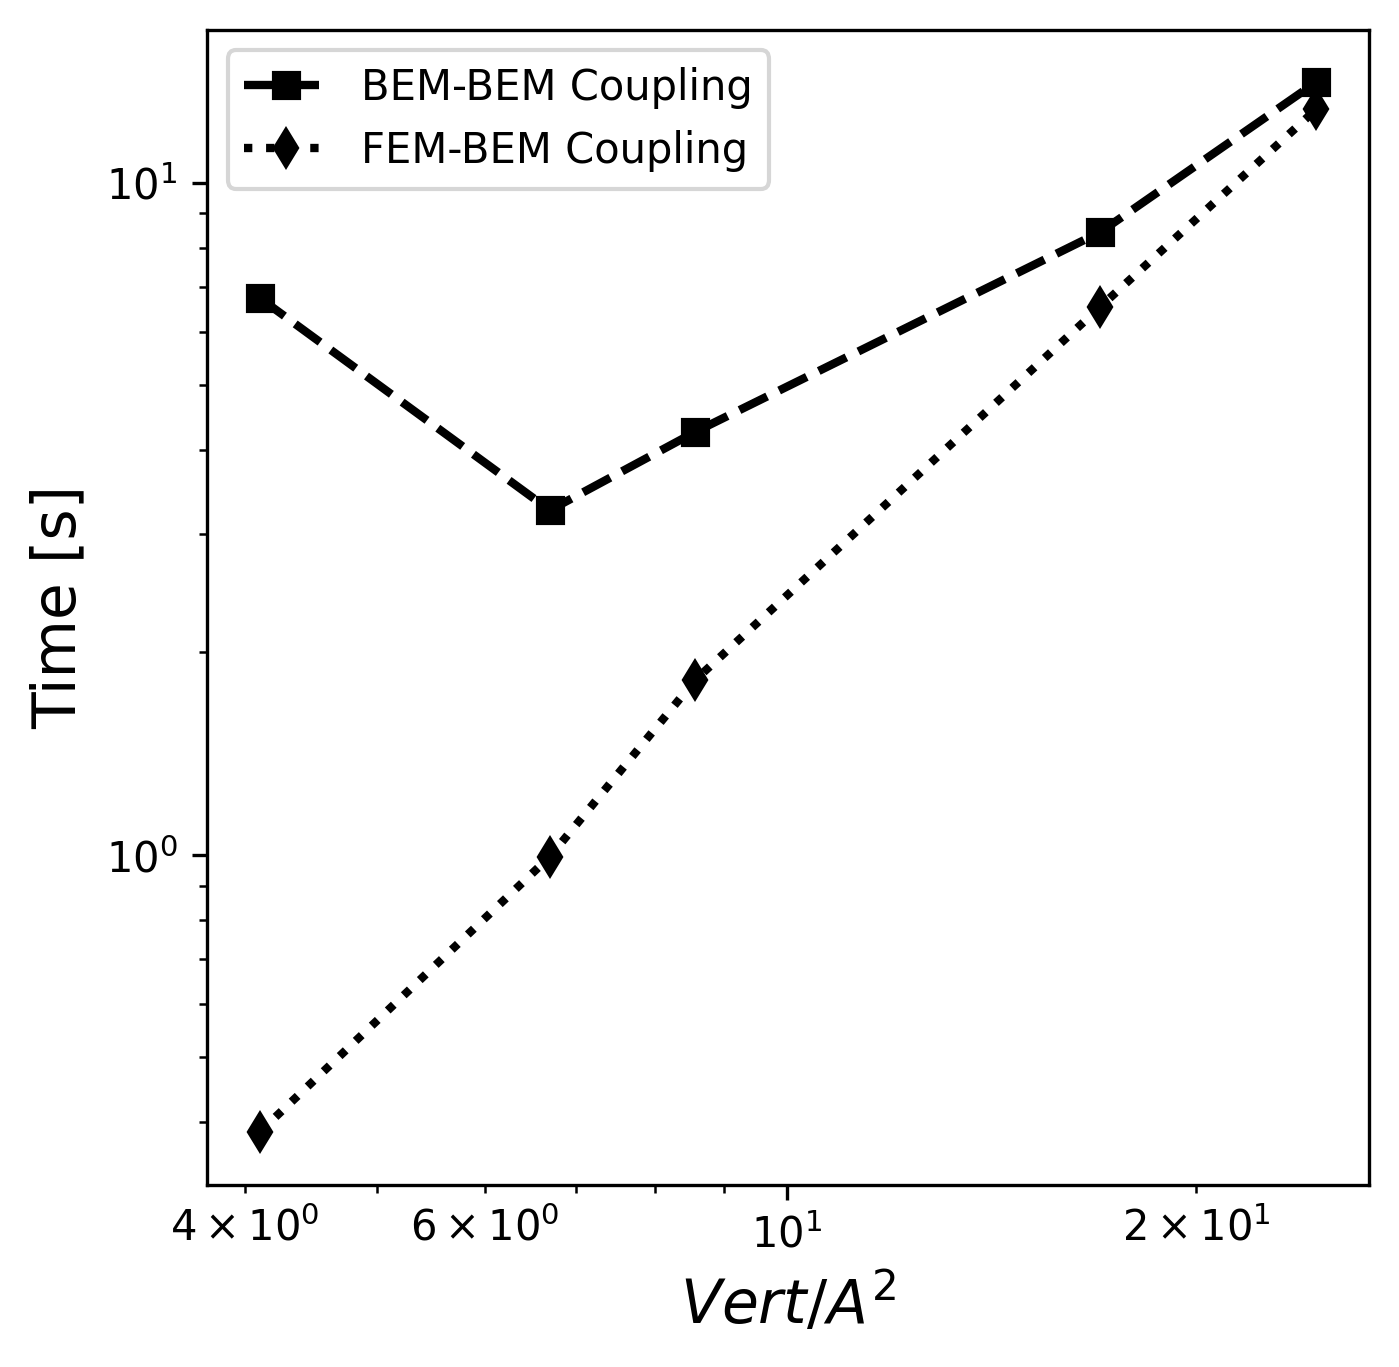
\includegraphics[width=0.45\linewidth]{DolfinX_Arginine2_const_coeff_total_time.png}
%   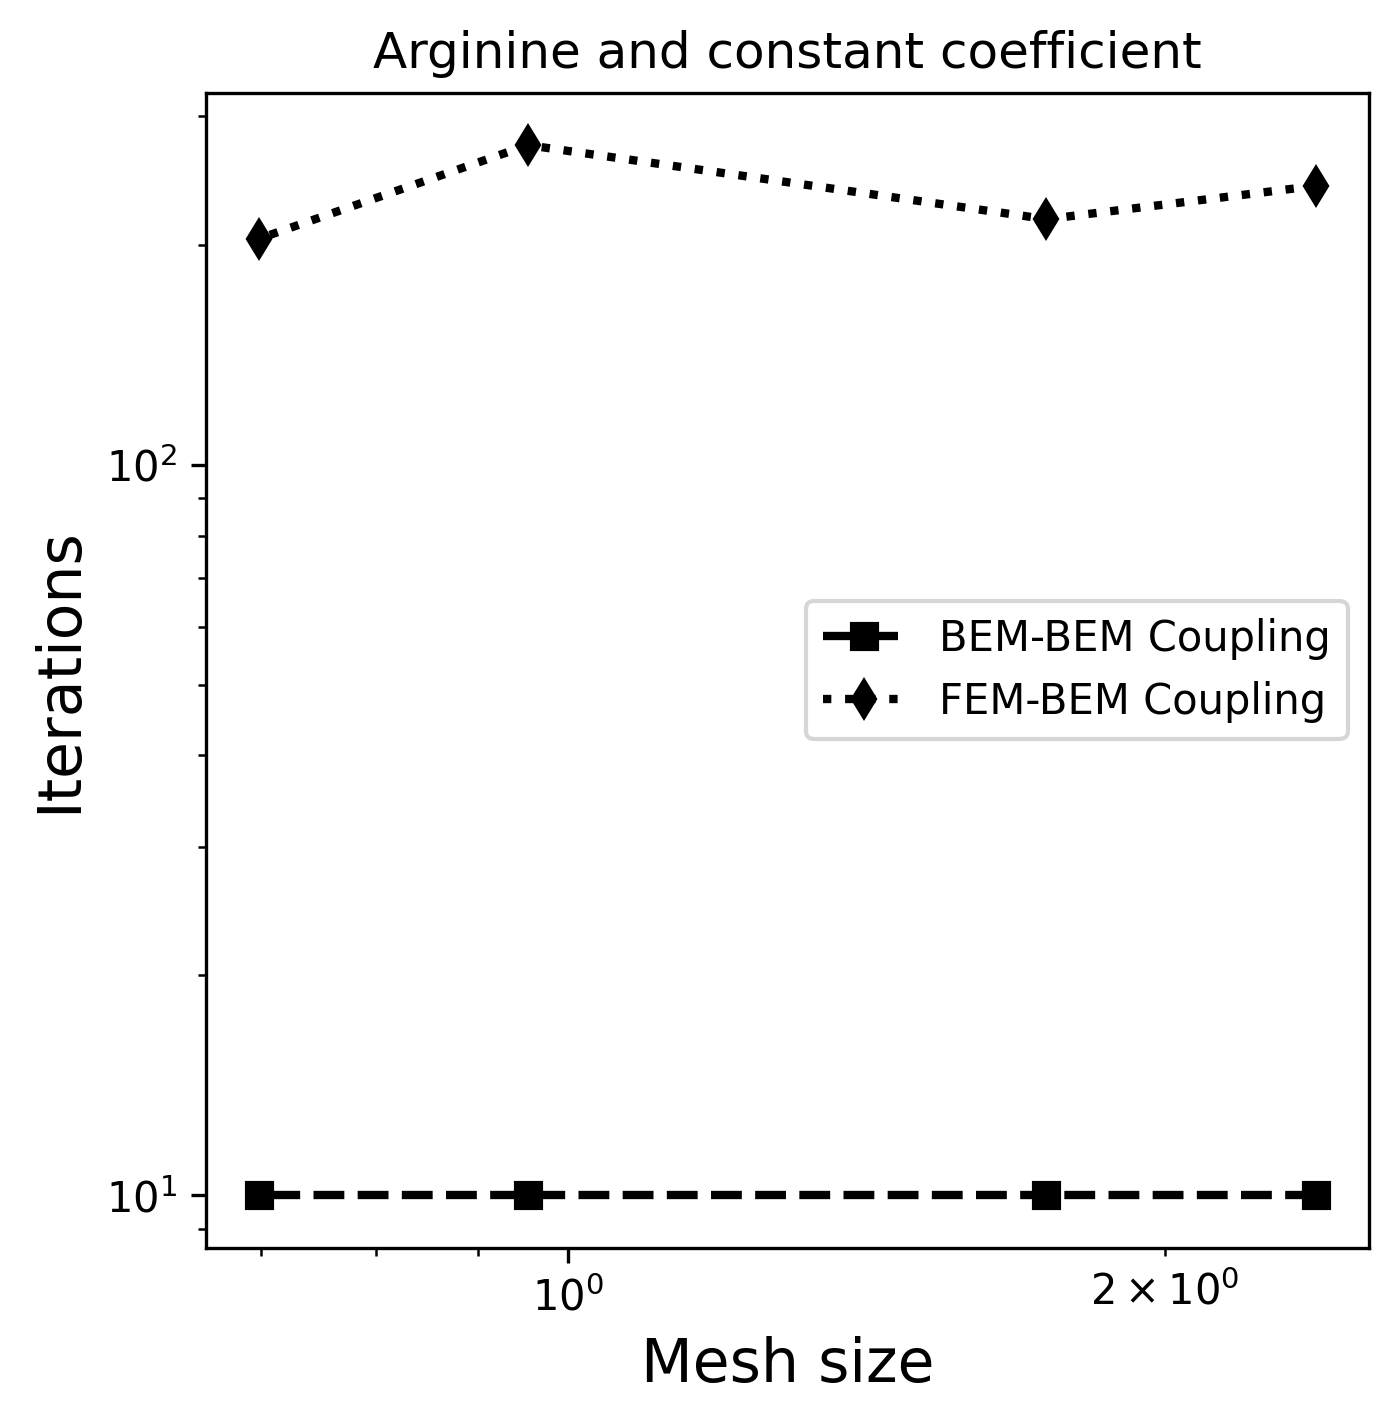
\includegraphics[width=0.45\linewidth]{DolfinX_Arginine_const_coeff_iter_11.png}
%%  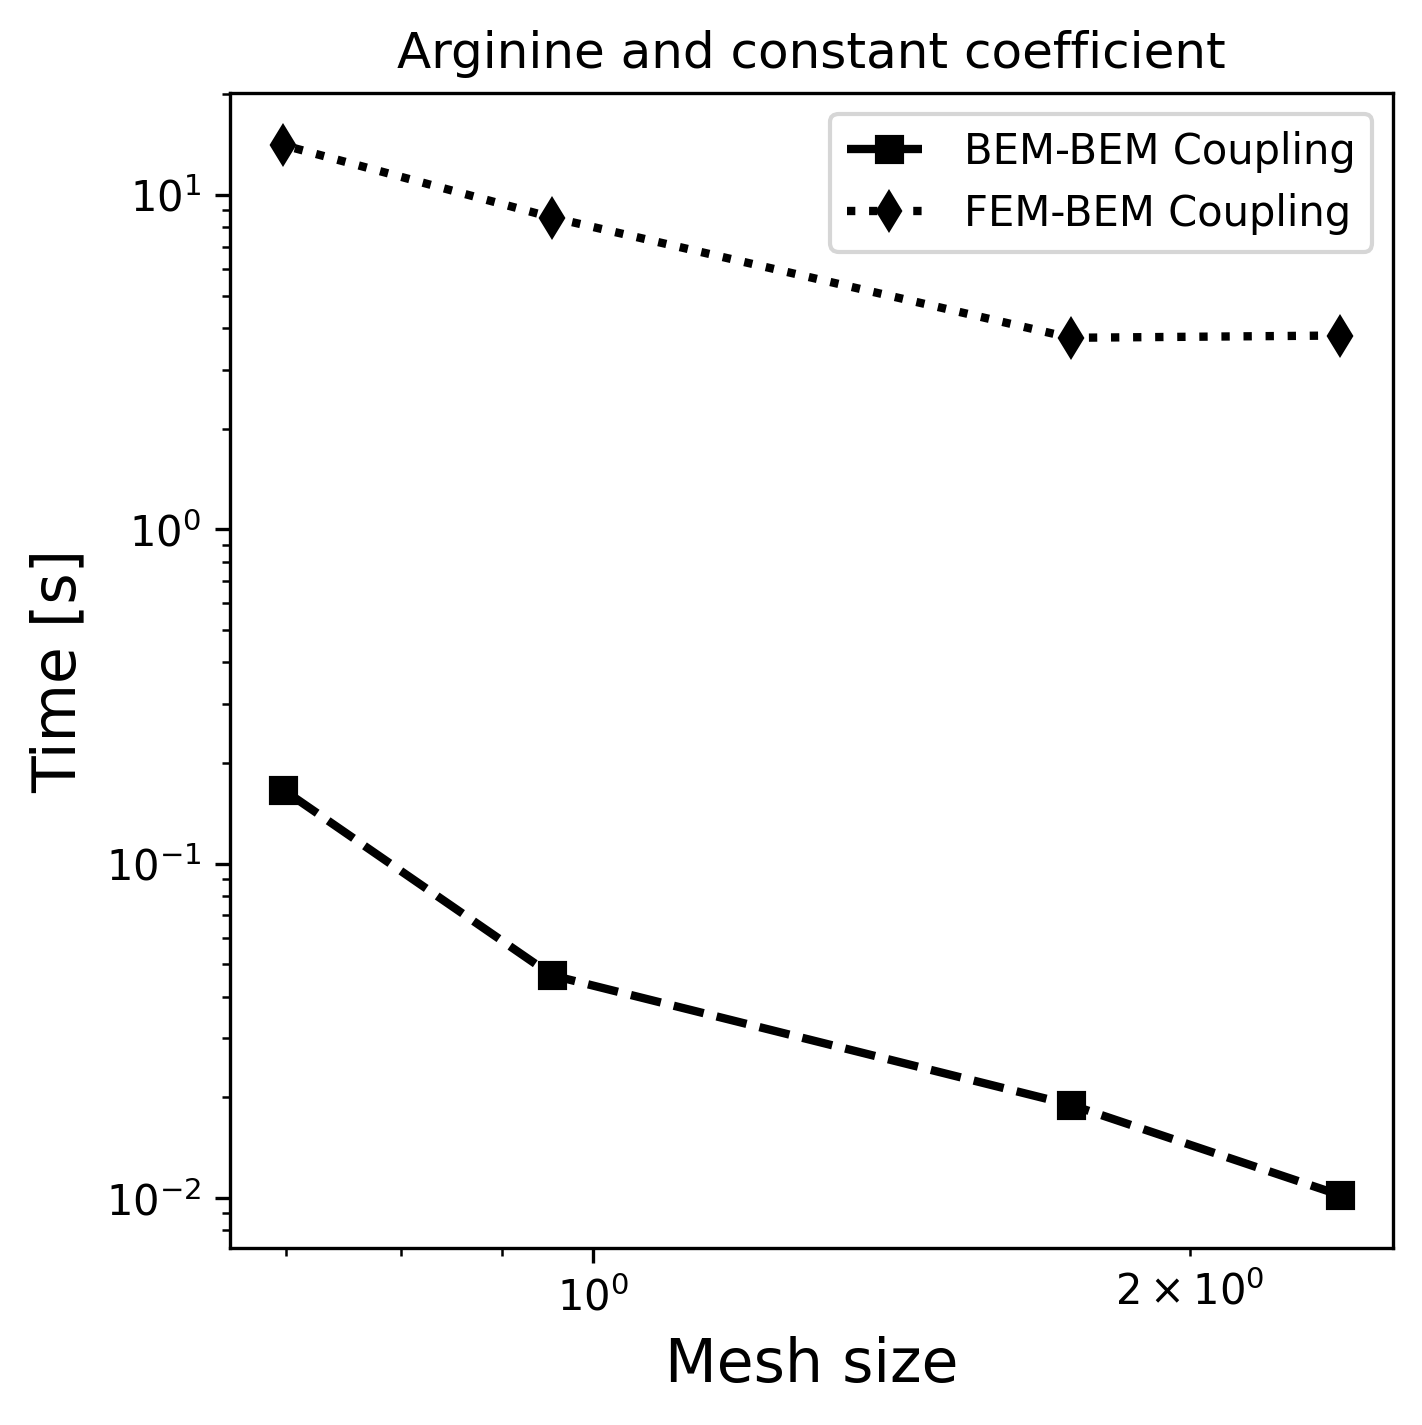
\includegraphics[width=0.45\linewidth]{DolfinX_Arginine_const_coeff_time_11.png}
%%  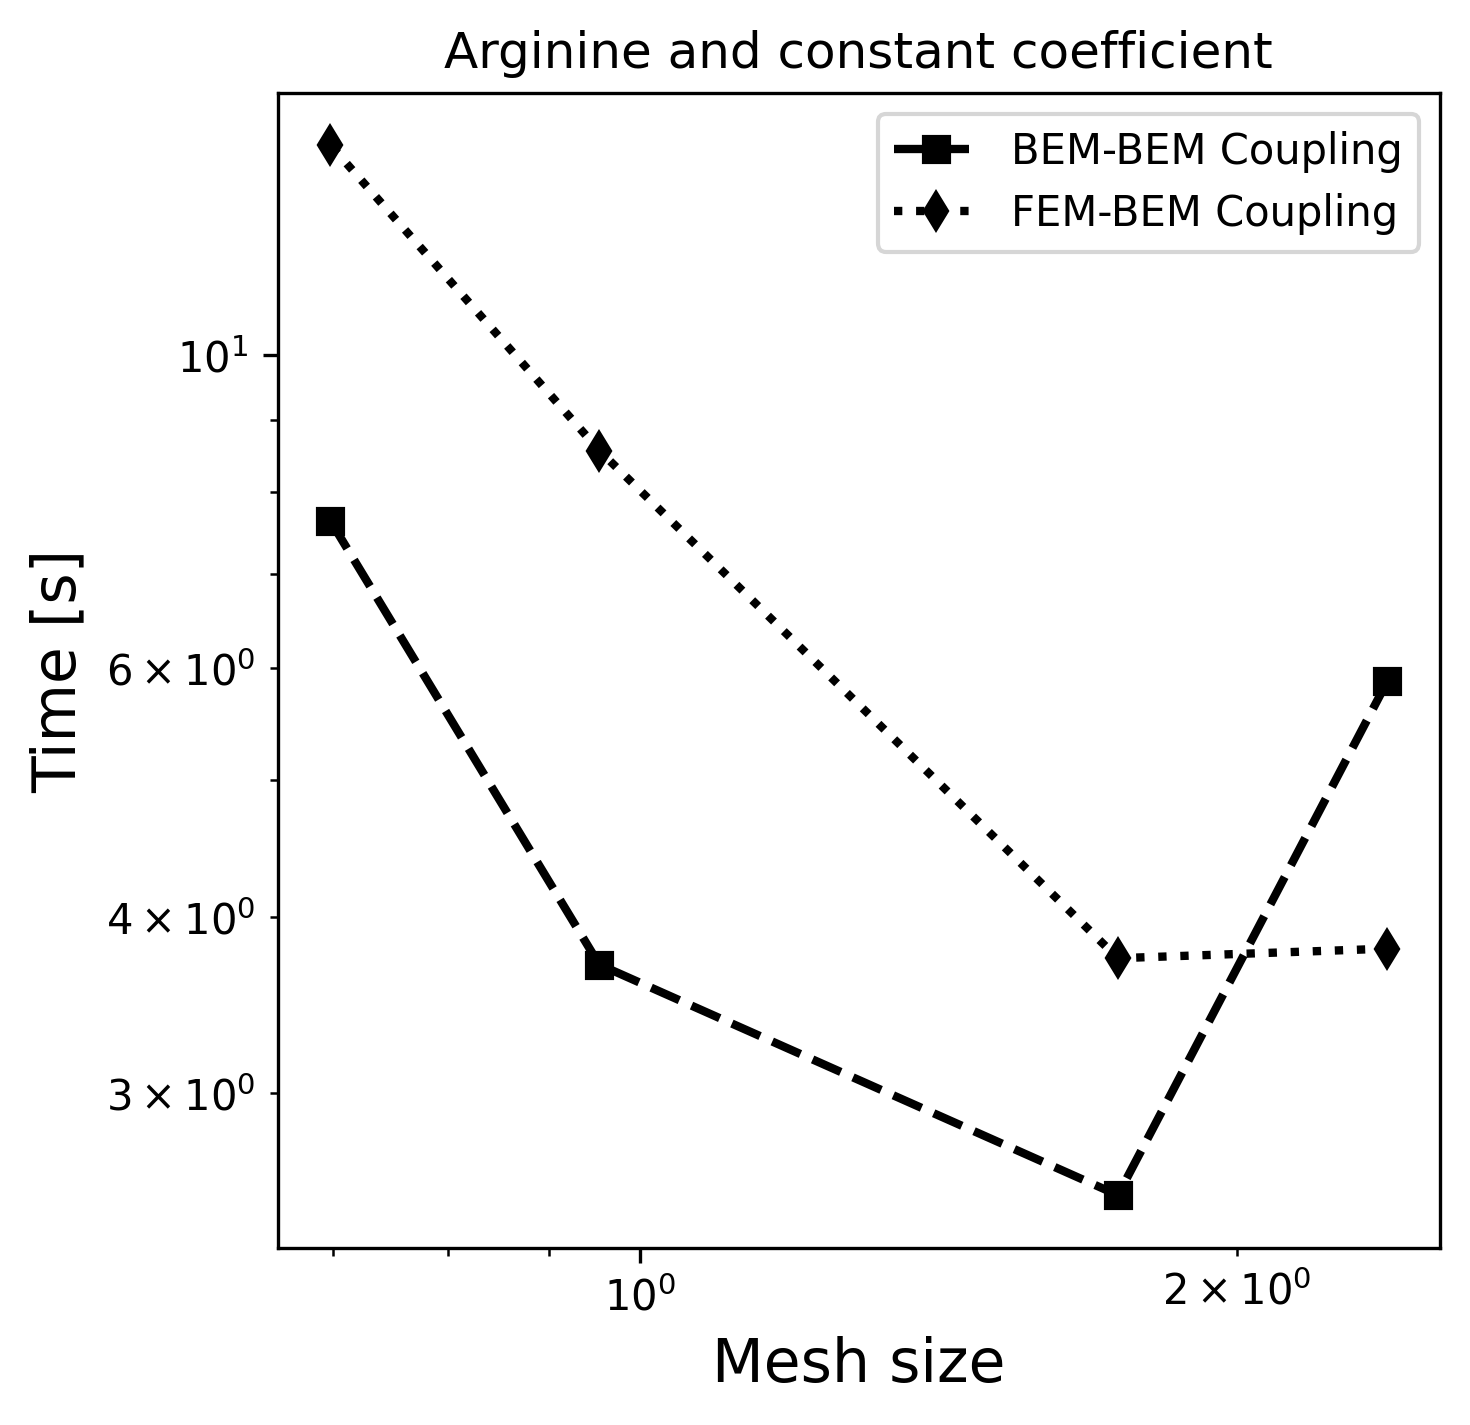
\includegraphics[width=0.45\linewidth]{DolfinX_Arginine_const_coeff_setup_time_11.png}
%  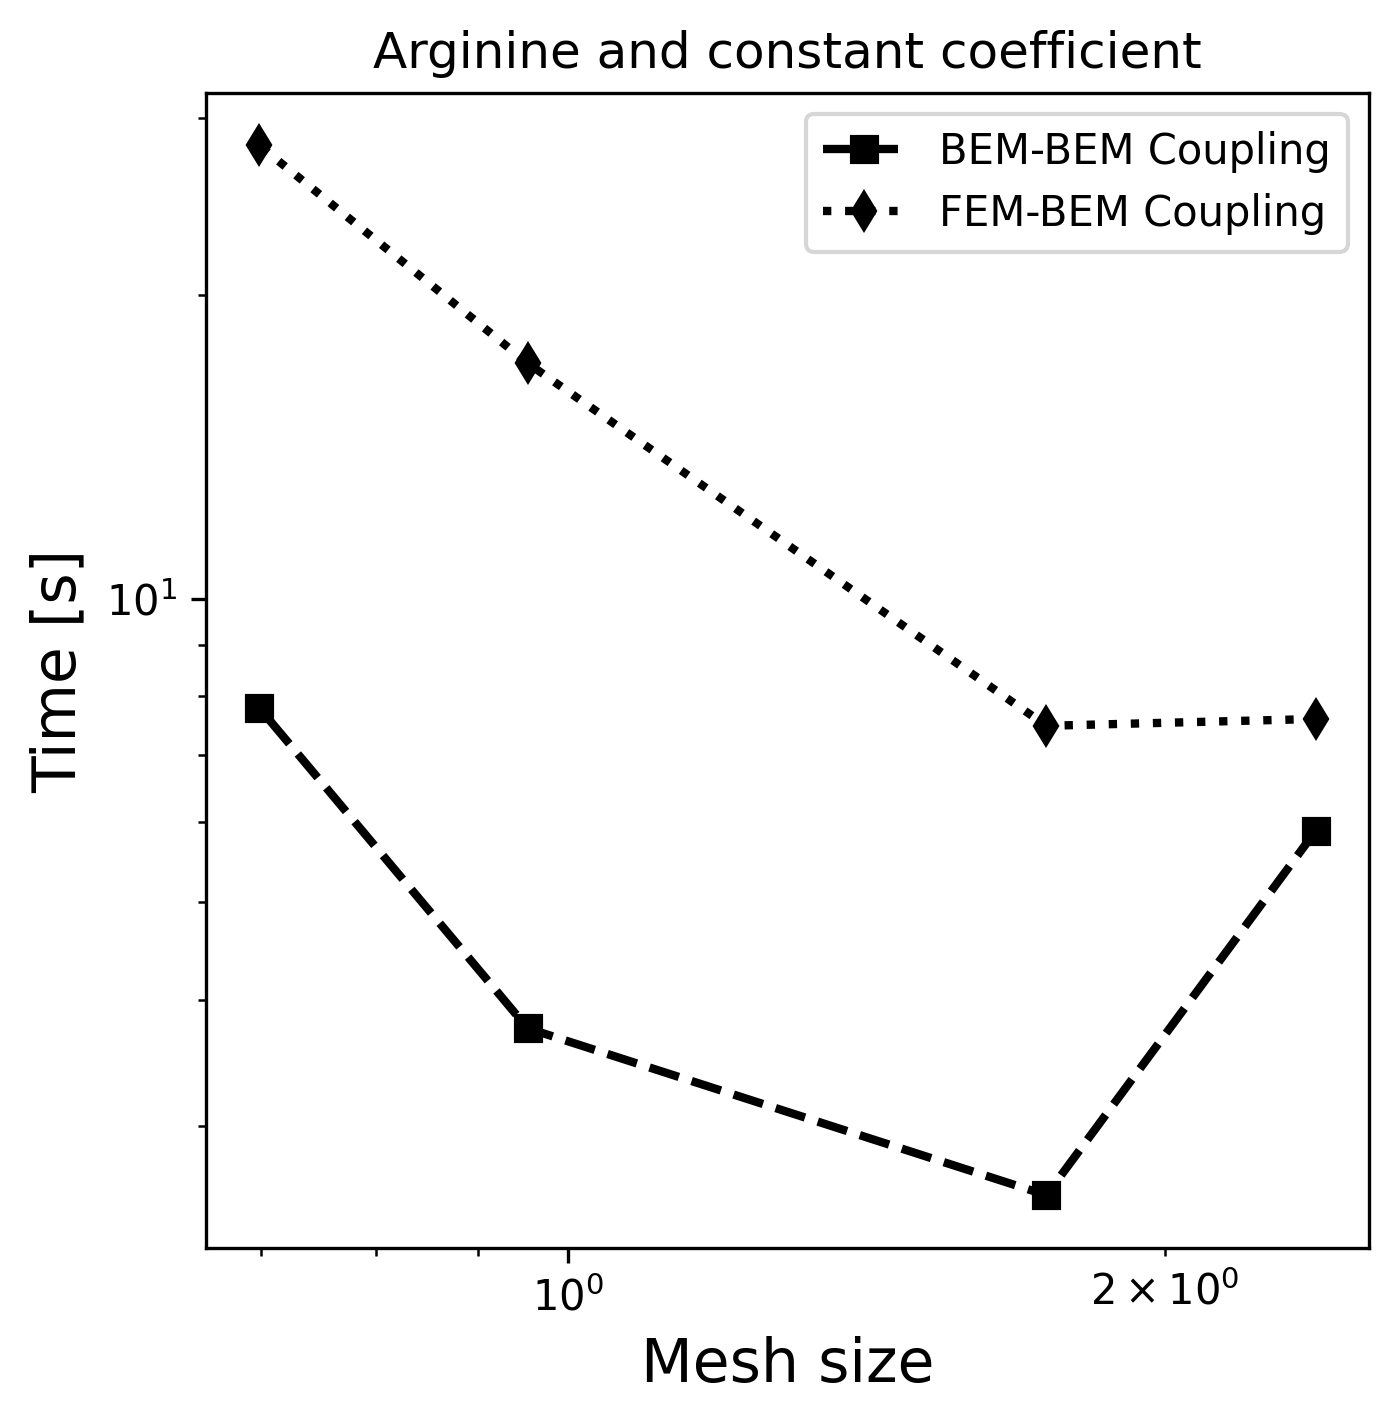
\includegraphics[width=0.45\linewidth]{DolfinX_Arginine_const_coeff_total_time_11.png}
  \caption{Iteration count (left) and time-to-solution (right) for Arginine with a constant permittivity. %(left: Online time taken to solve systems, right: Offline time taken to set up systems). 
%NOTE: x axis differ between top and bottom. Also, should we include preconditioned vs non preconditioned? We could easily precondition BEM-BEM too.  %(1) fix title, (2) can we put them in a single plot, (3) 
%maybe we could also add a "error" wrt extrapolation, or a plot with energy for each mesh?
}
\label{fig:arg2_constant_time_iter}
\end{figure}

%\begin{figure}
%\centering
%%   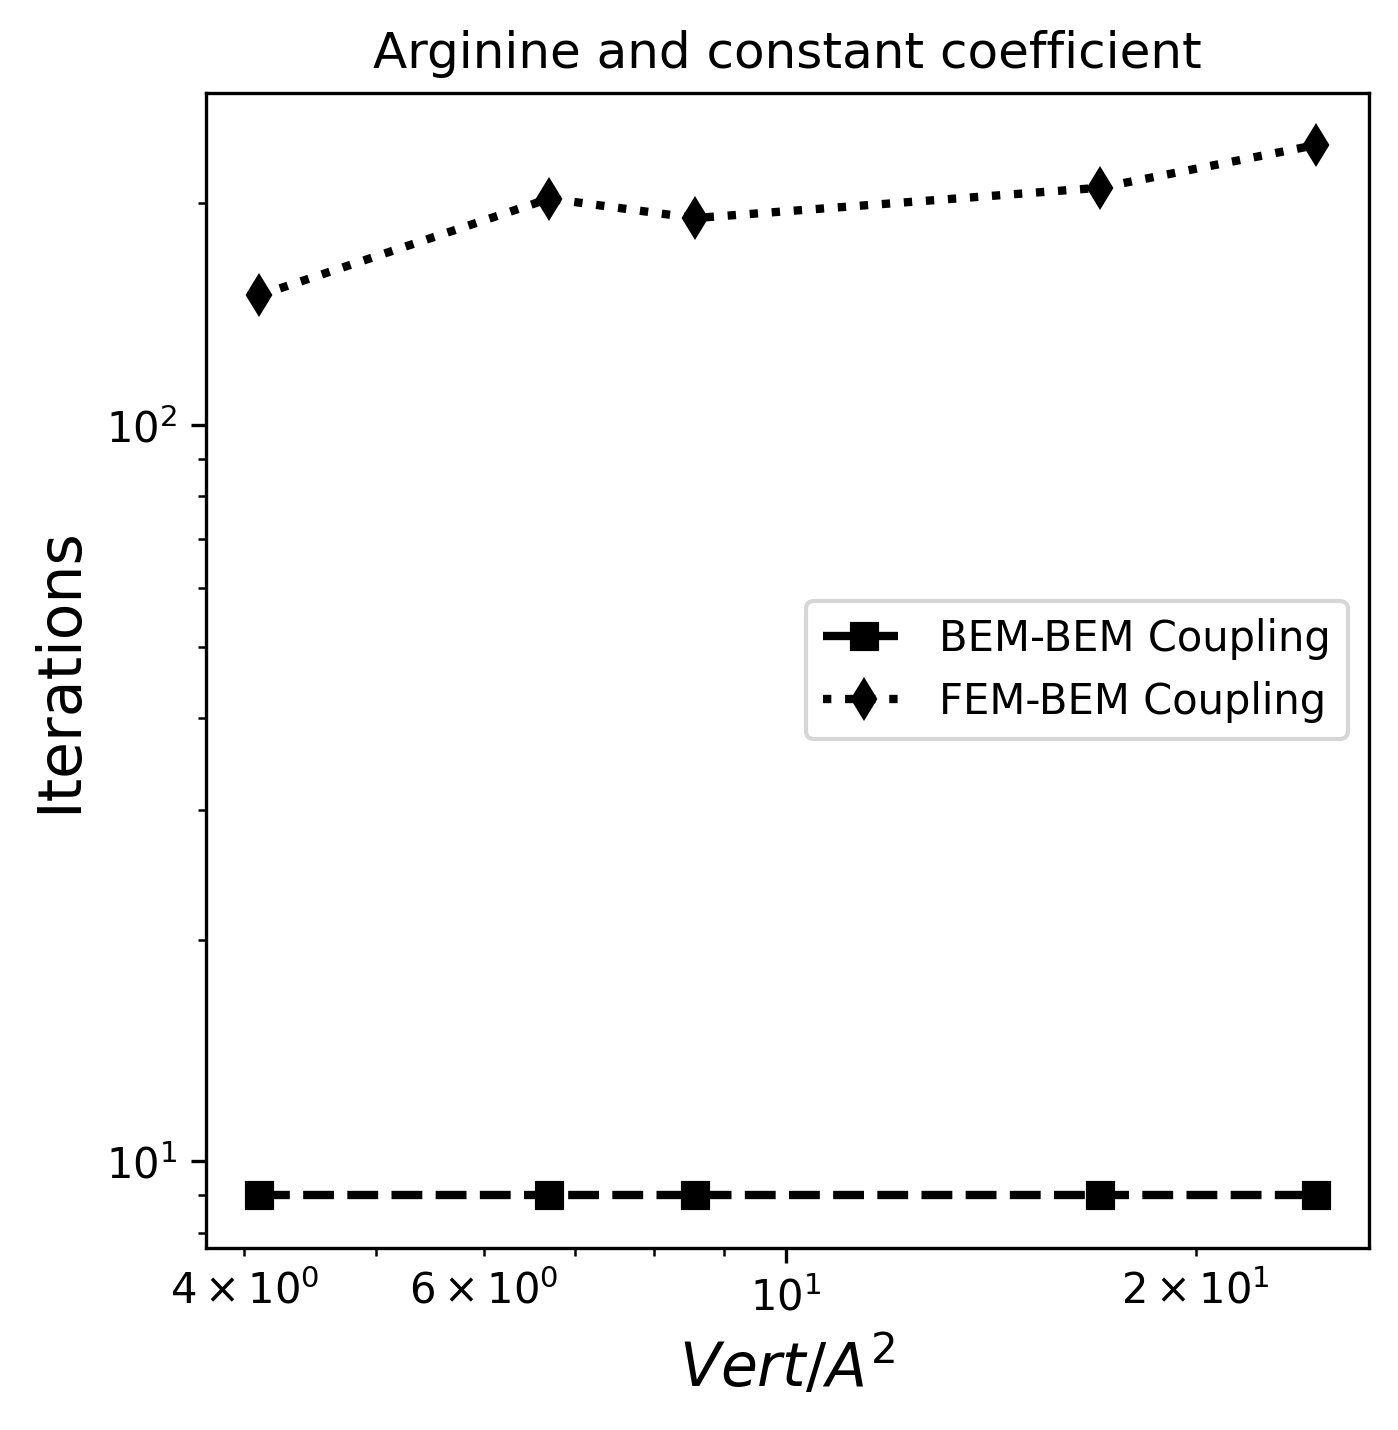
\includegraphics[width=0.45\linewidth]{DolfinX_Arginine2_const_coeff_iter.png}
%%%  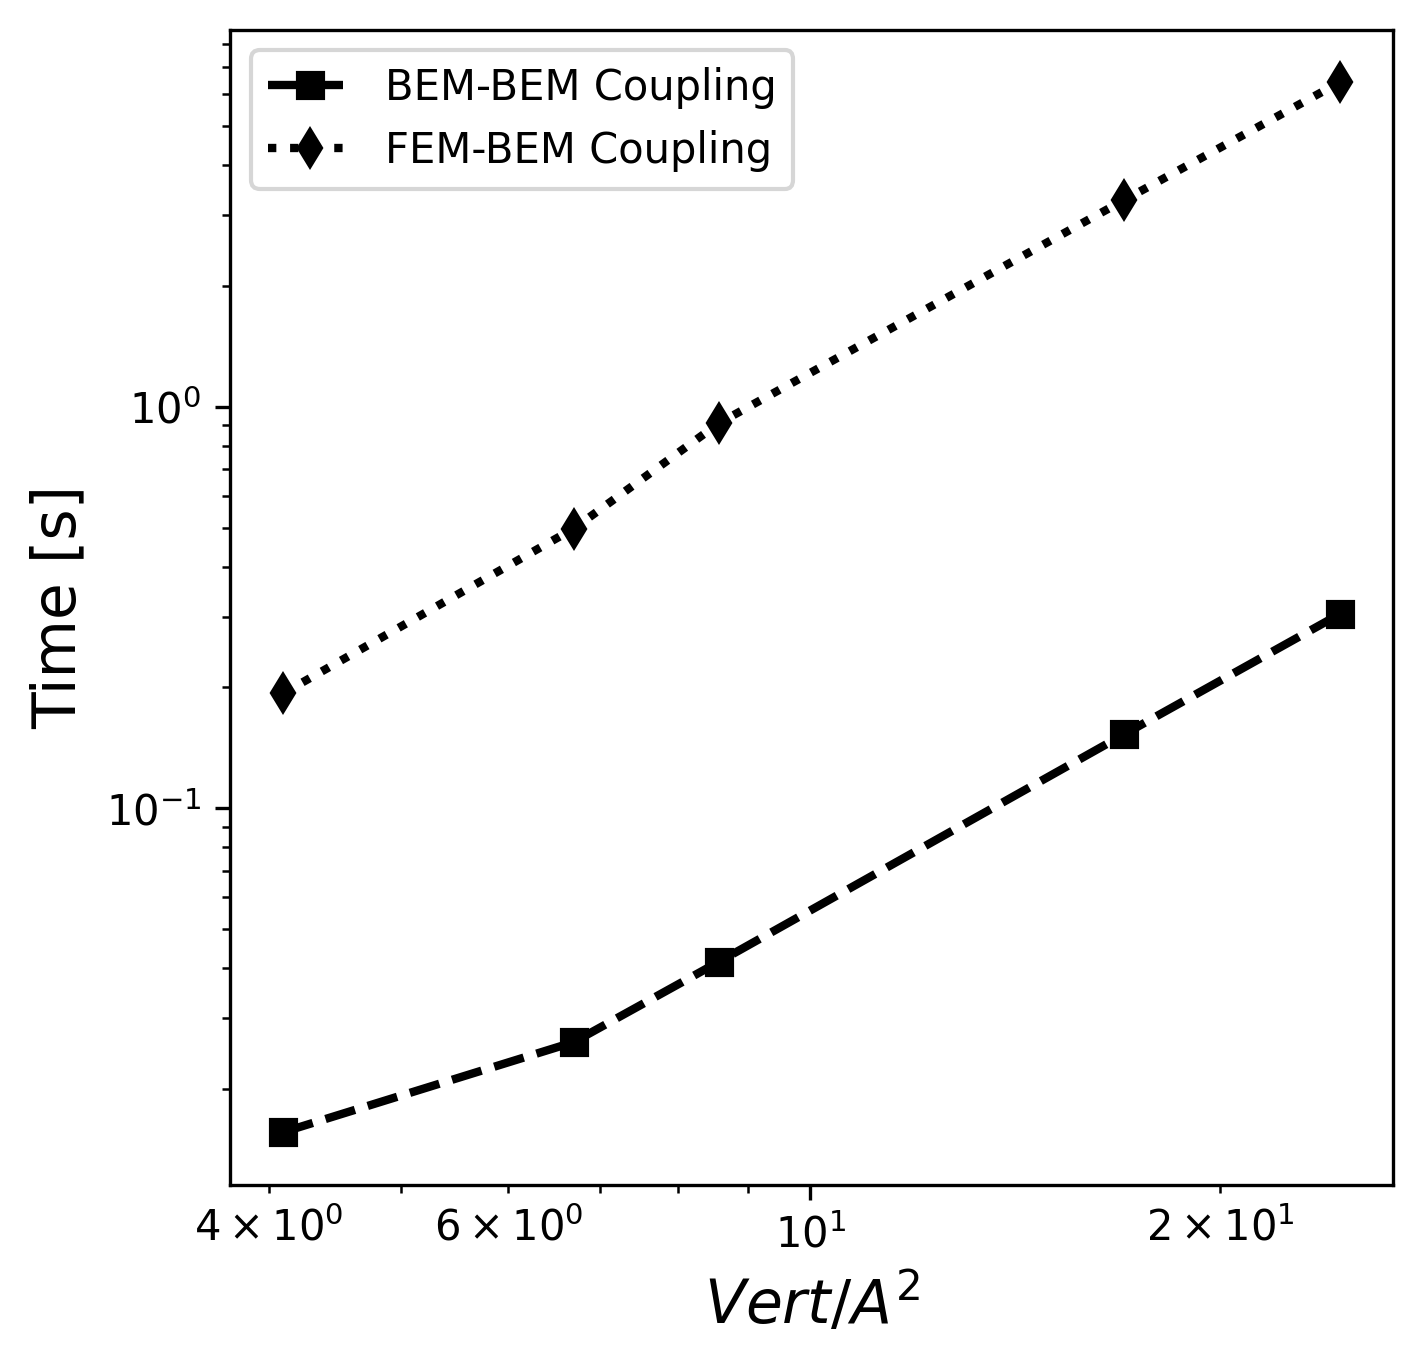
\includegraphics[width=0.45\linewidth]{DolfinX_Arginine2_const_coeff_time.png}
%%%  \includegraphics[width=0.45\linewidth]{DolfinX_Arginine2_const_coeff_setup_time.png}
%%  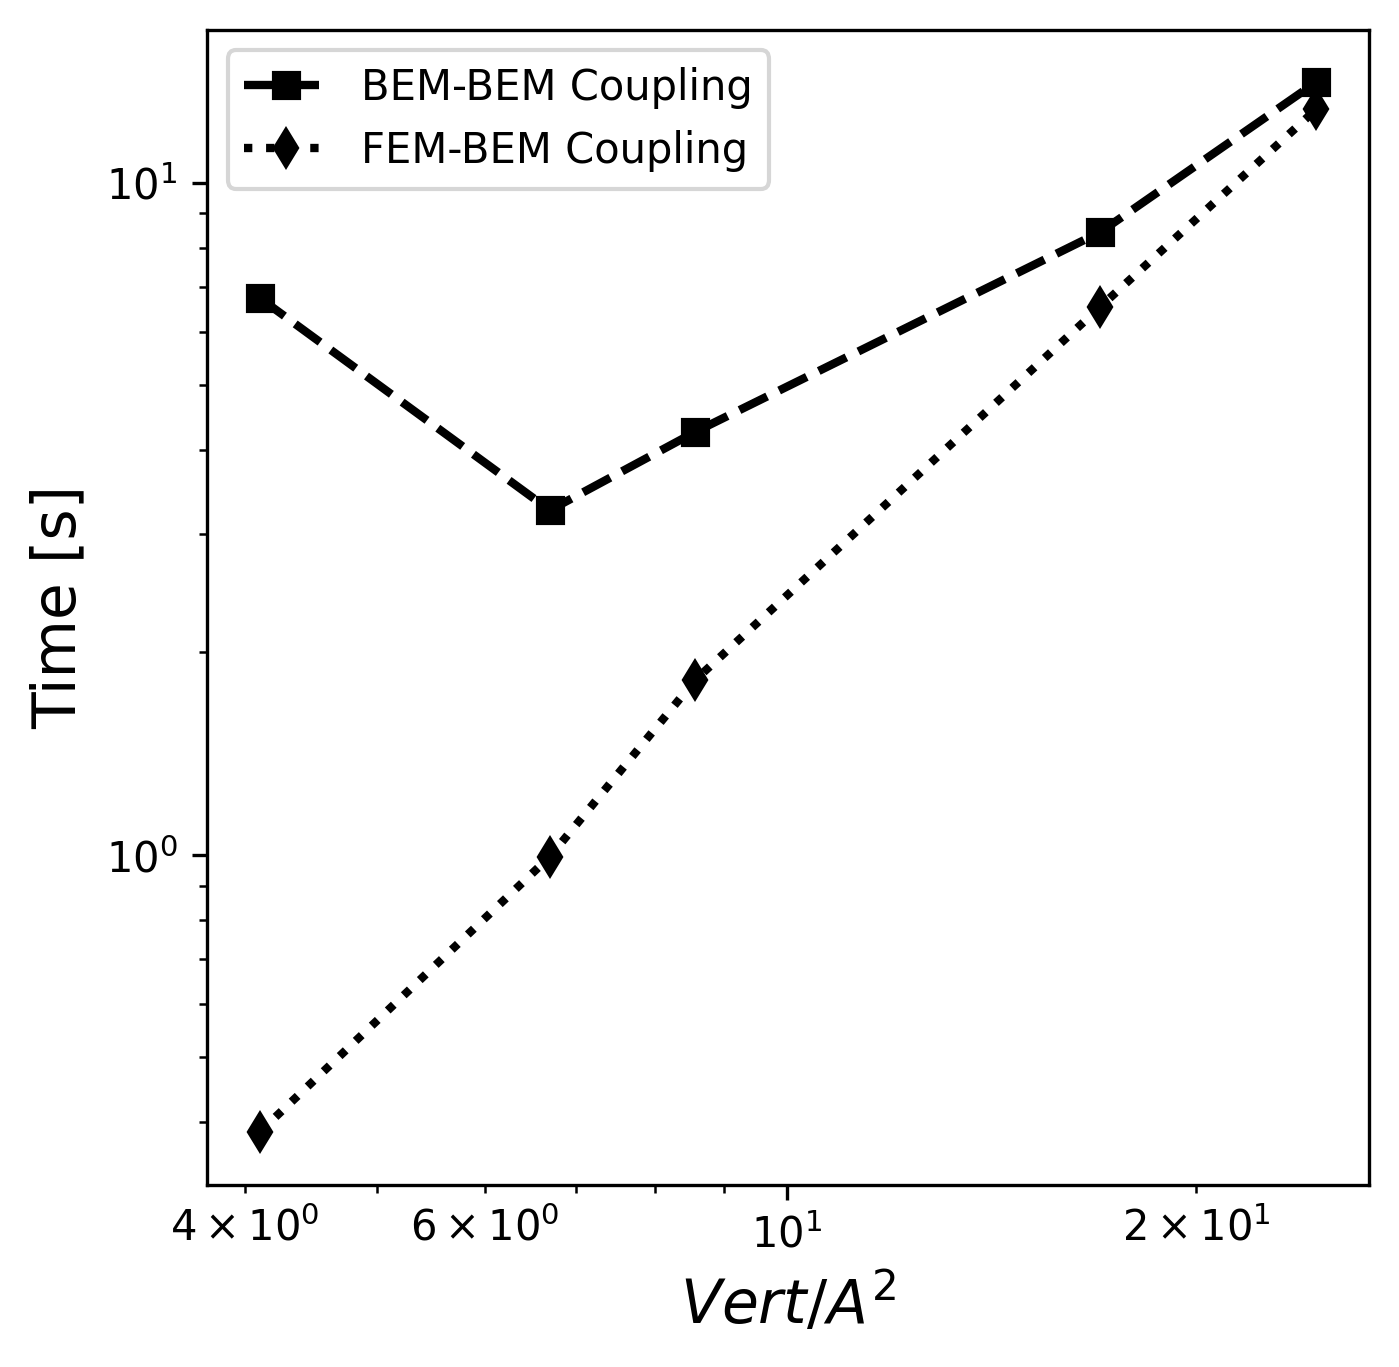
\includegraphics[width=0.45\linewidth]{DolfinX_Arginine2_const_coeff_total_time.png}
%   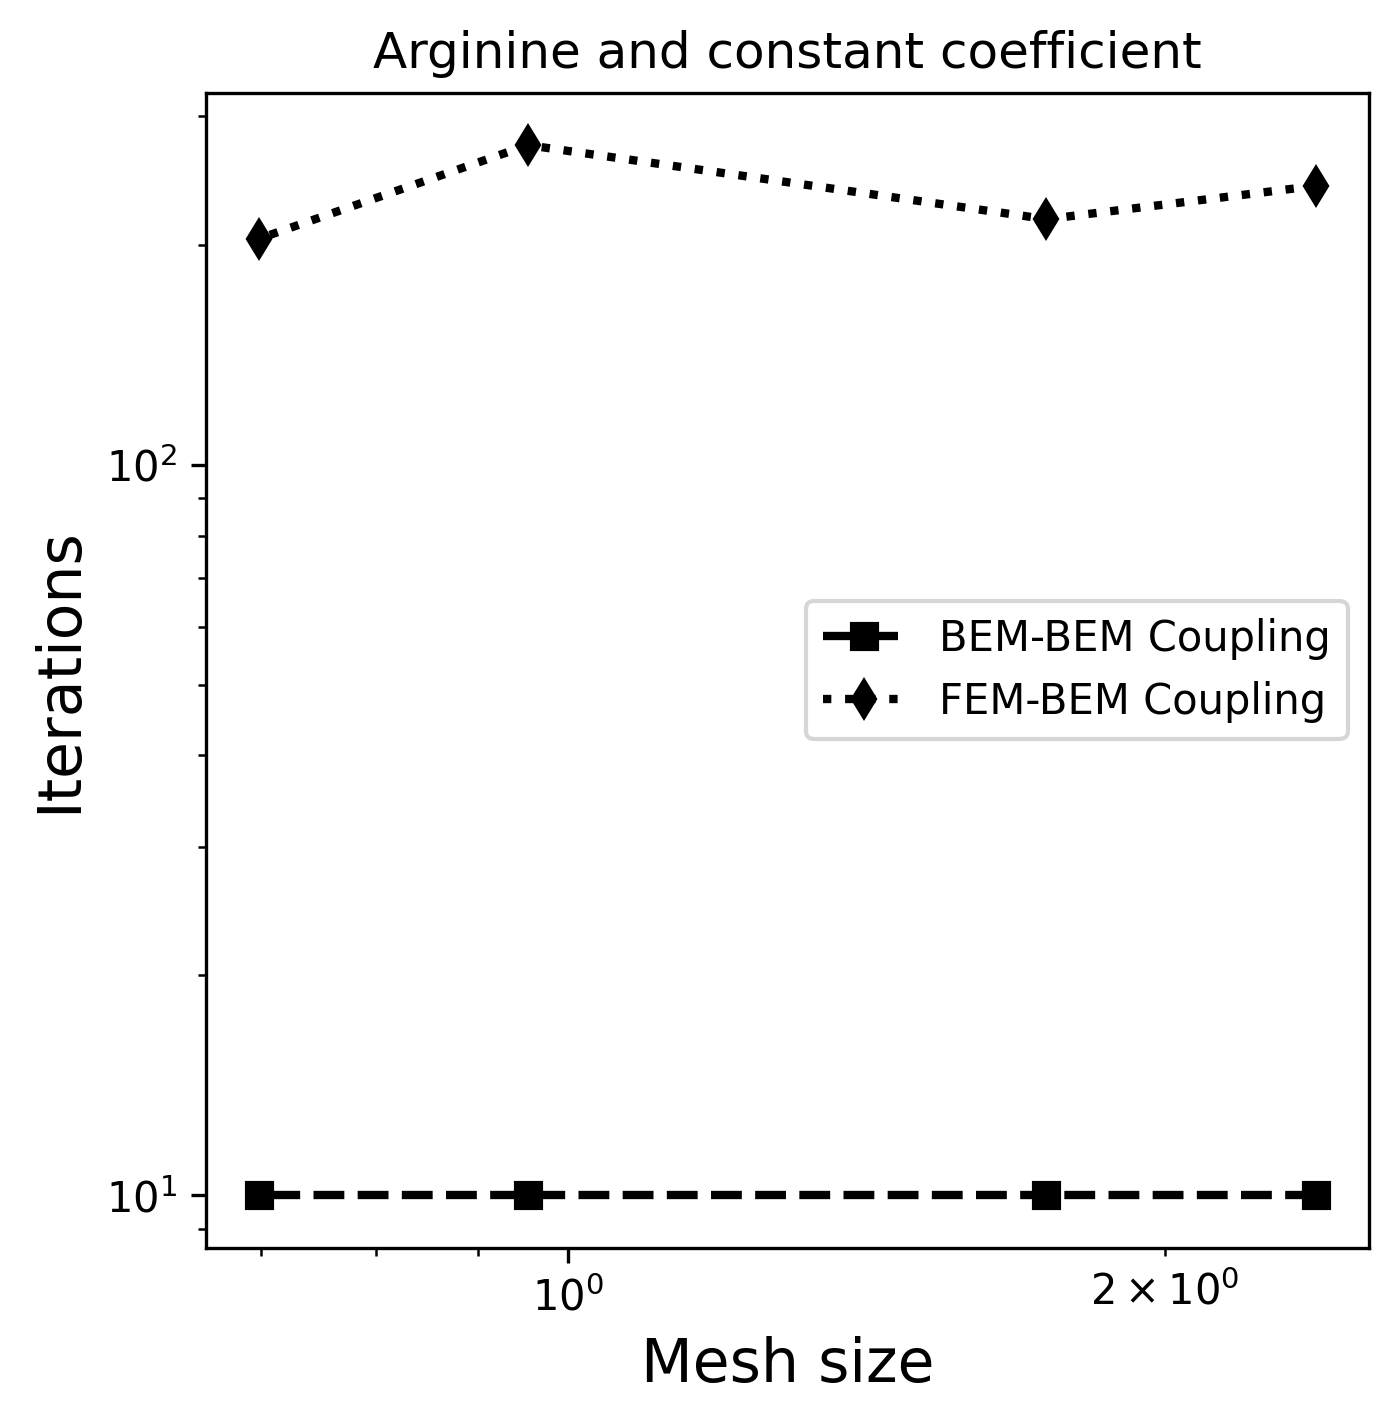
\includegraphics[width=0.45\linewidth]{DolfinX_Arginine_const_coeff_iter_11.png}
%%  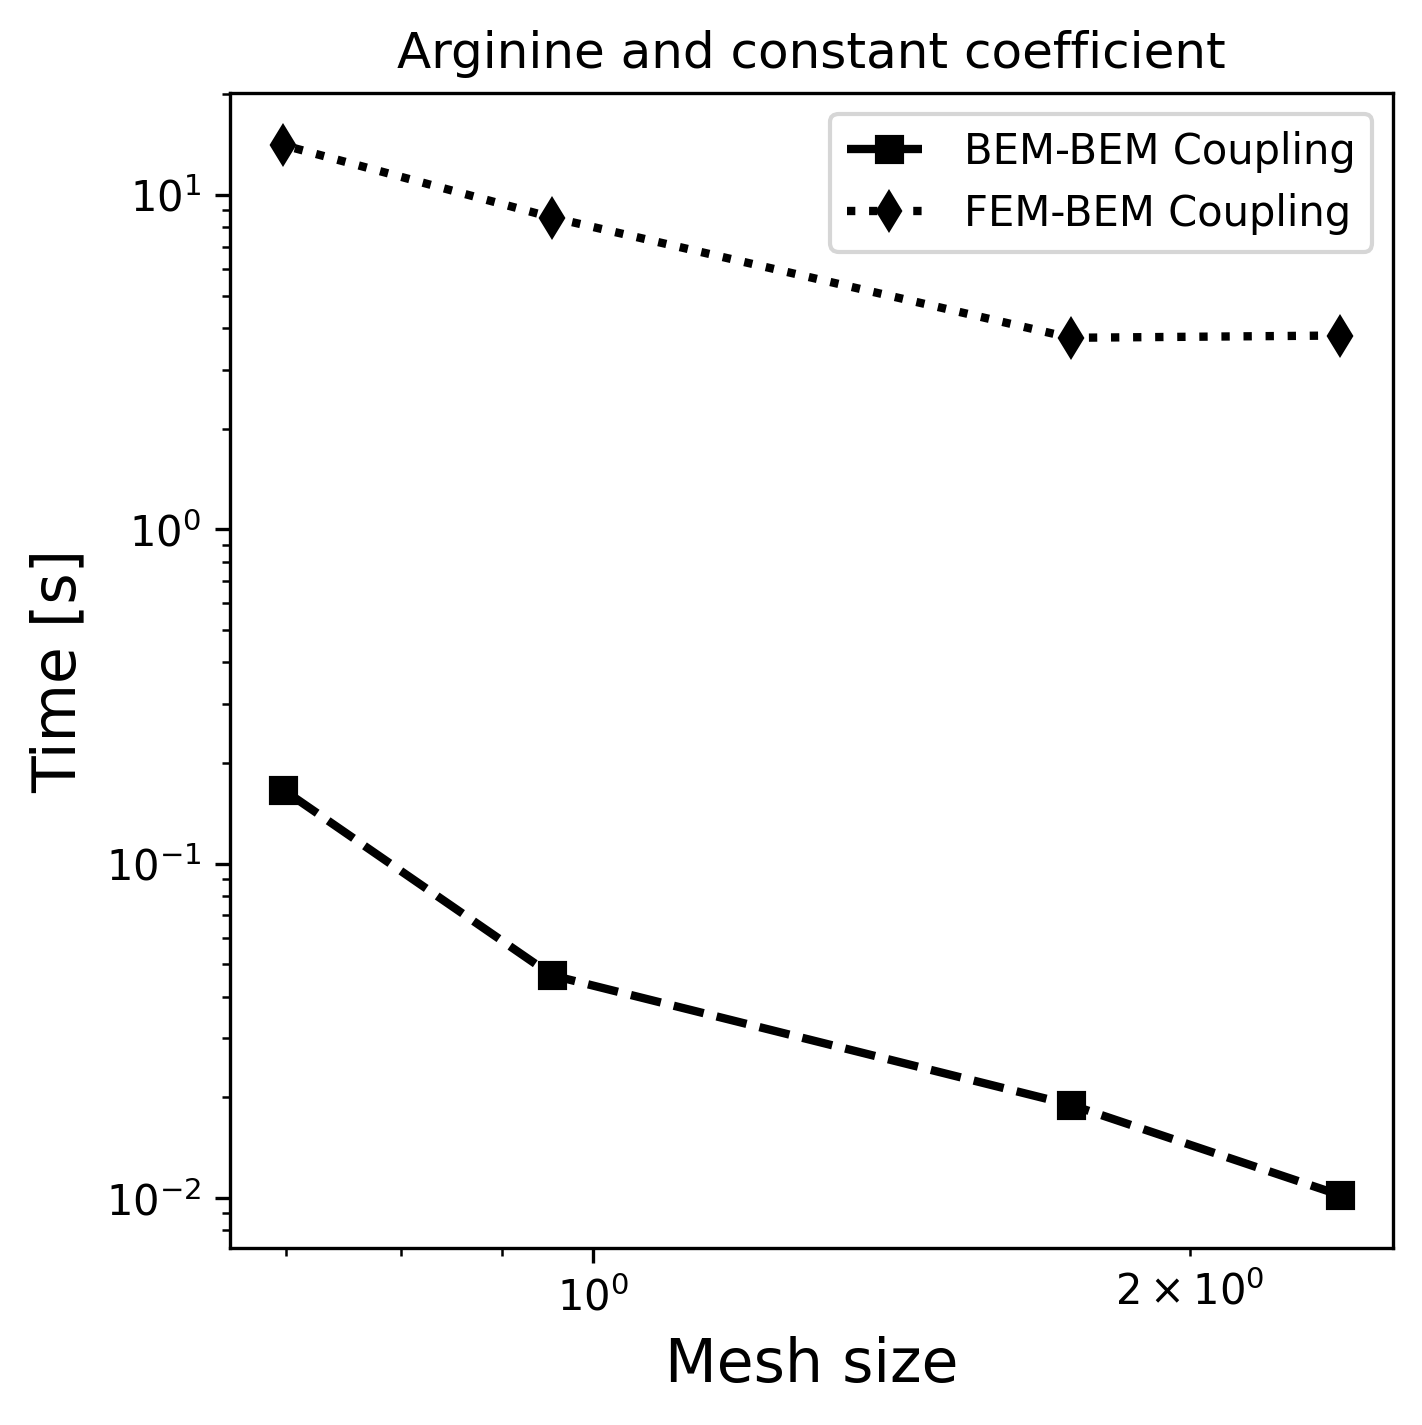
\includegraphics[width=0.45\linewidth]{DolfinX_Arginine_const_coeff_time_11.png}
%%  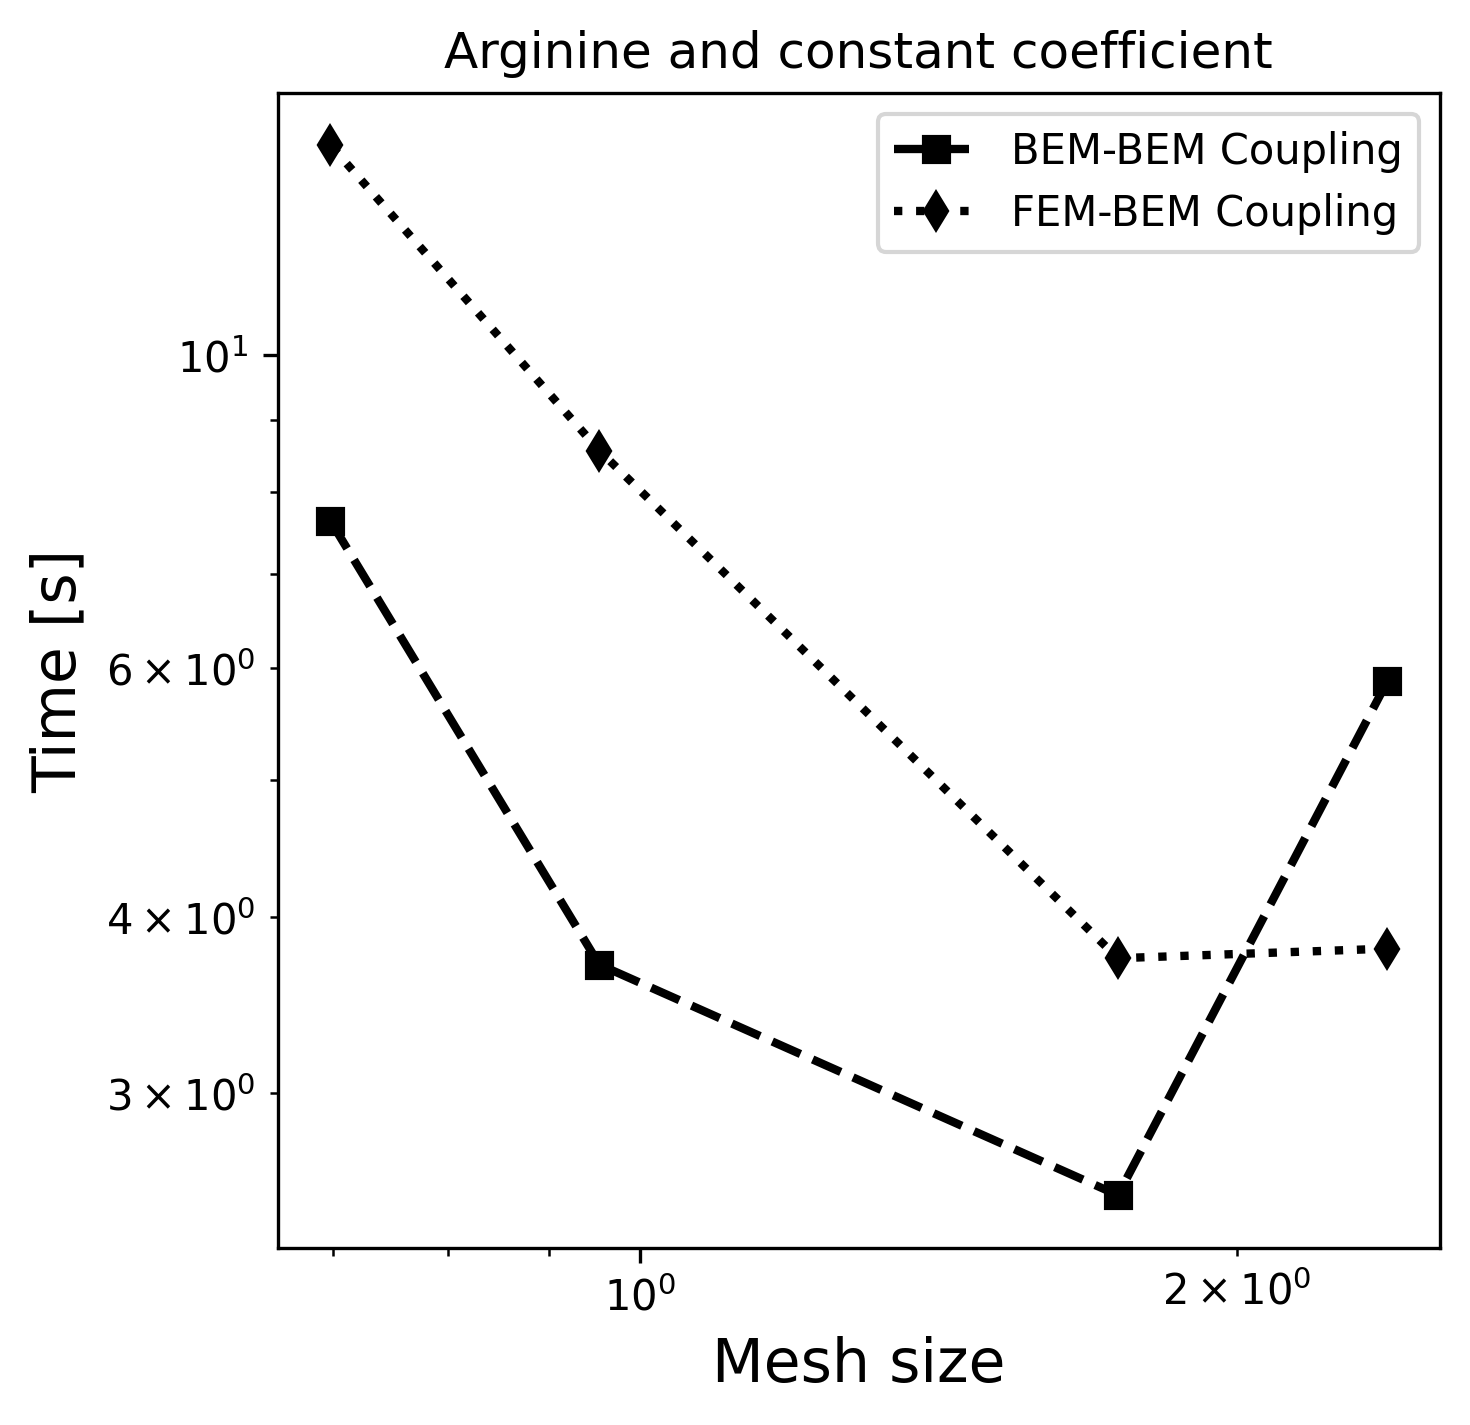
\includegraphics[width=0.45\linewidth]{DolfinX_Arginine_const_coeff_setup_time_11.png}
%  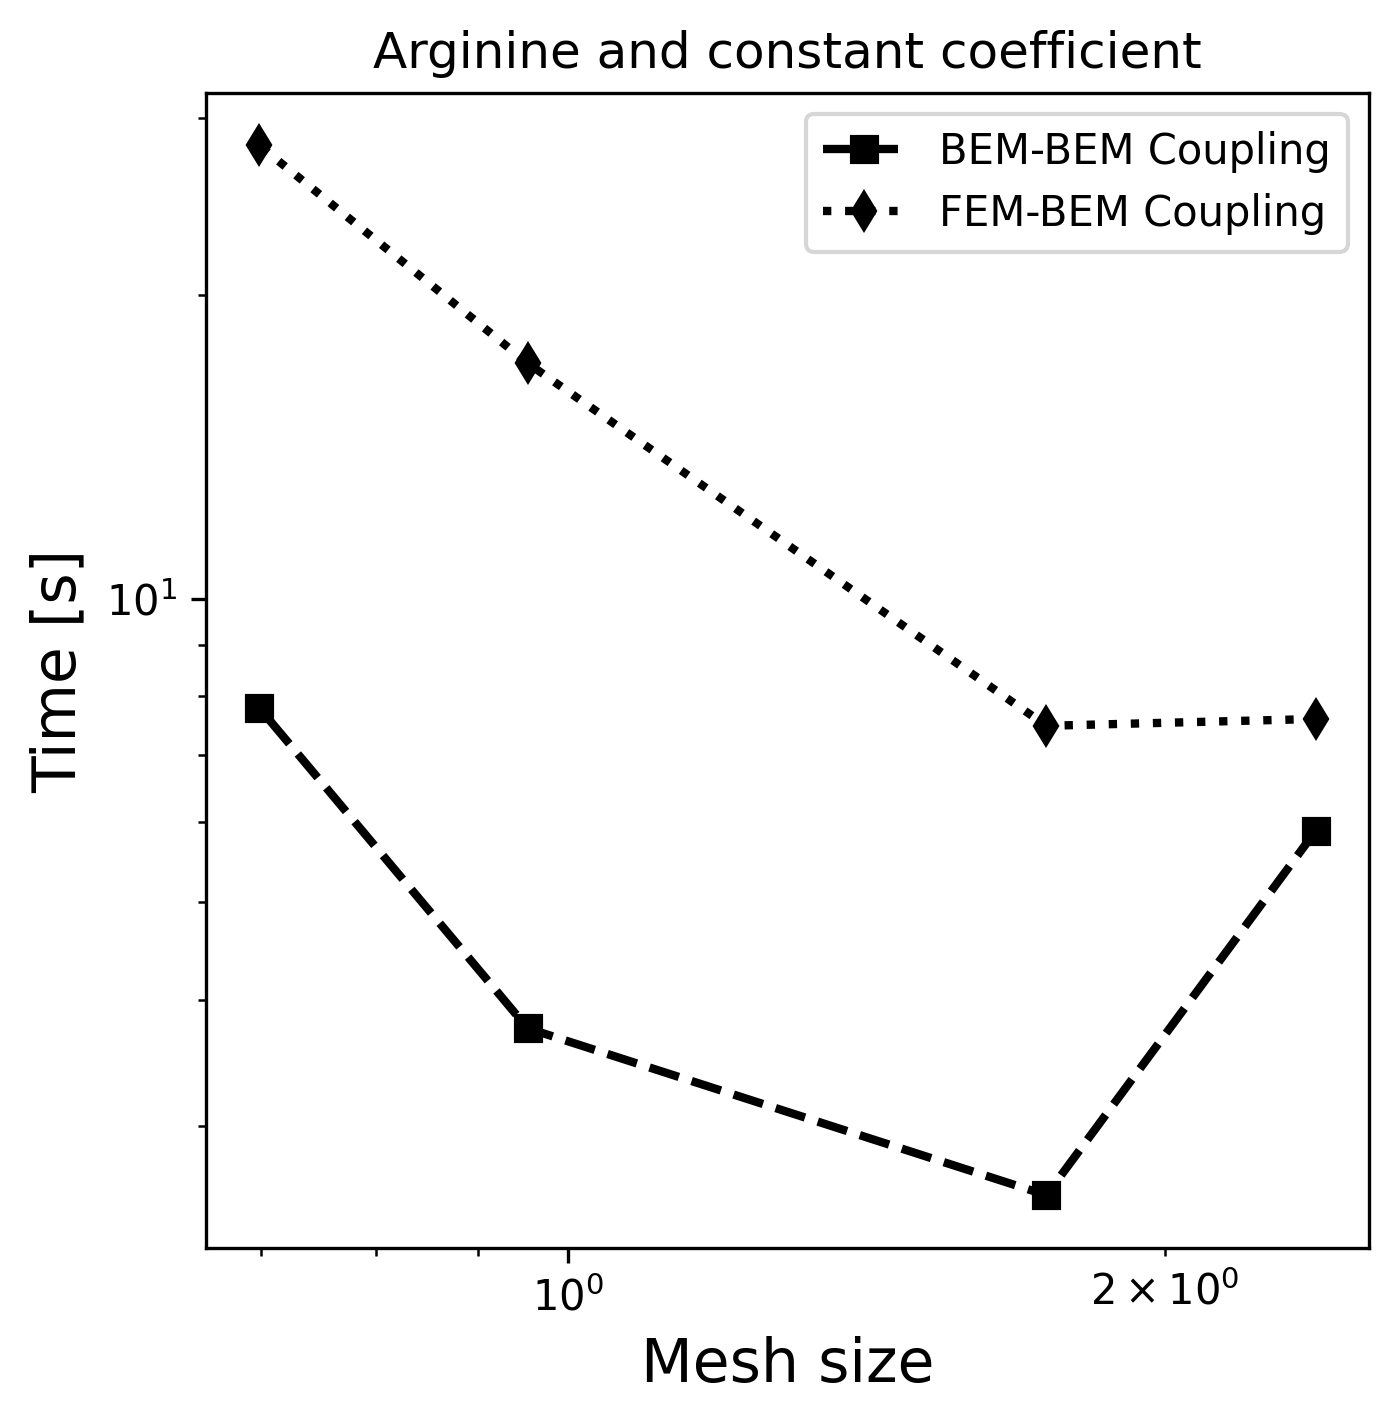
\includegraphics[width=0.45\linewidth]{DolfinX_Arginine_const_coeff_total_time_11.png}
%  \caption{Iteration count (left) and time-to-solution (right) for Arginine with a constant permittivity. %(left: Online time taken to solve systems, right: Offline time taken to set up systems). 
%%NOTE: x axis differ between top and bottom. Also, should we include preconditioned vs non preconditioned? We could easily precondition BEM-BEM too.  %(1) fix title, (2) can we put them in a single plot, (3) 
%%maybe we could also add a "error" wrt extrapolation, or a plot with energy for each mesh?
%}
%\label{fig:arg_constant_time_iter}
%\end{figure}


%\begin{figure}
%\centering
%%   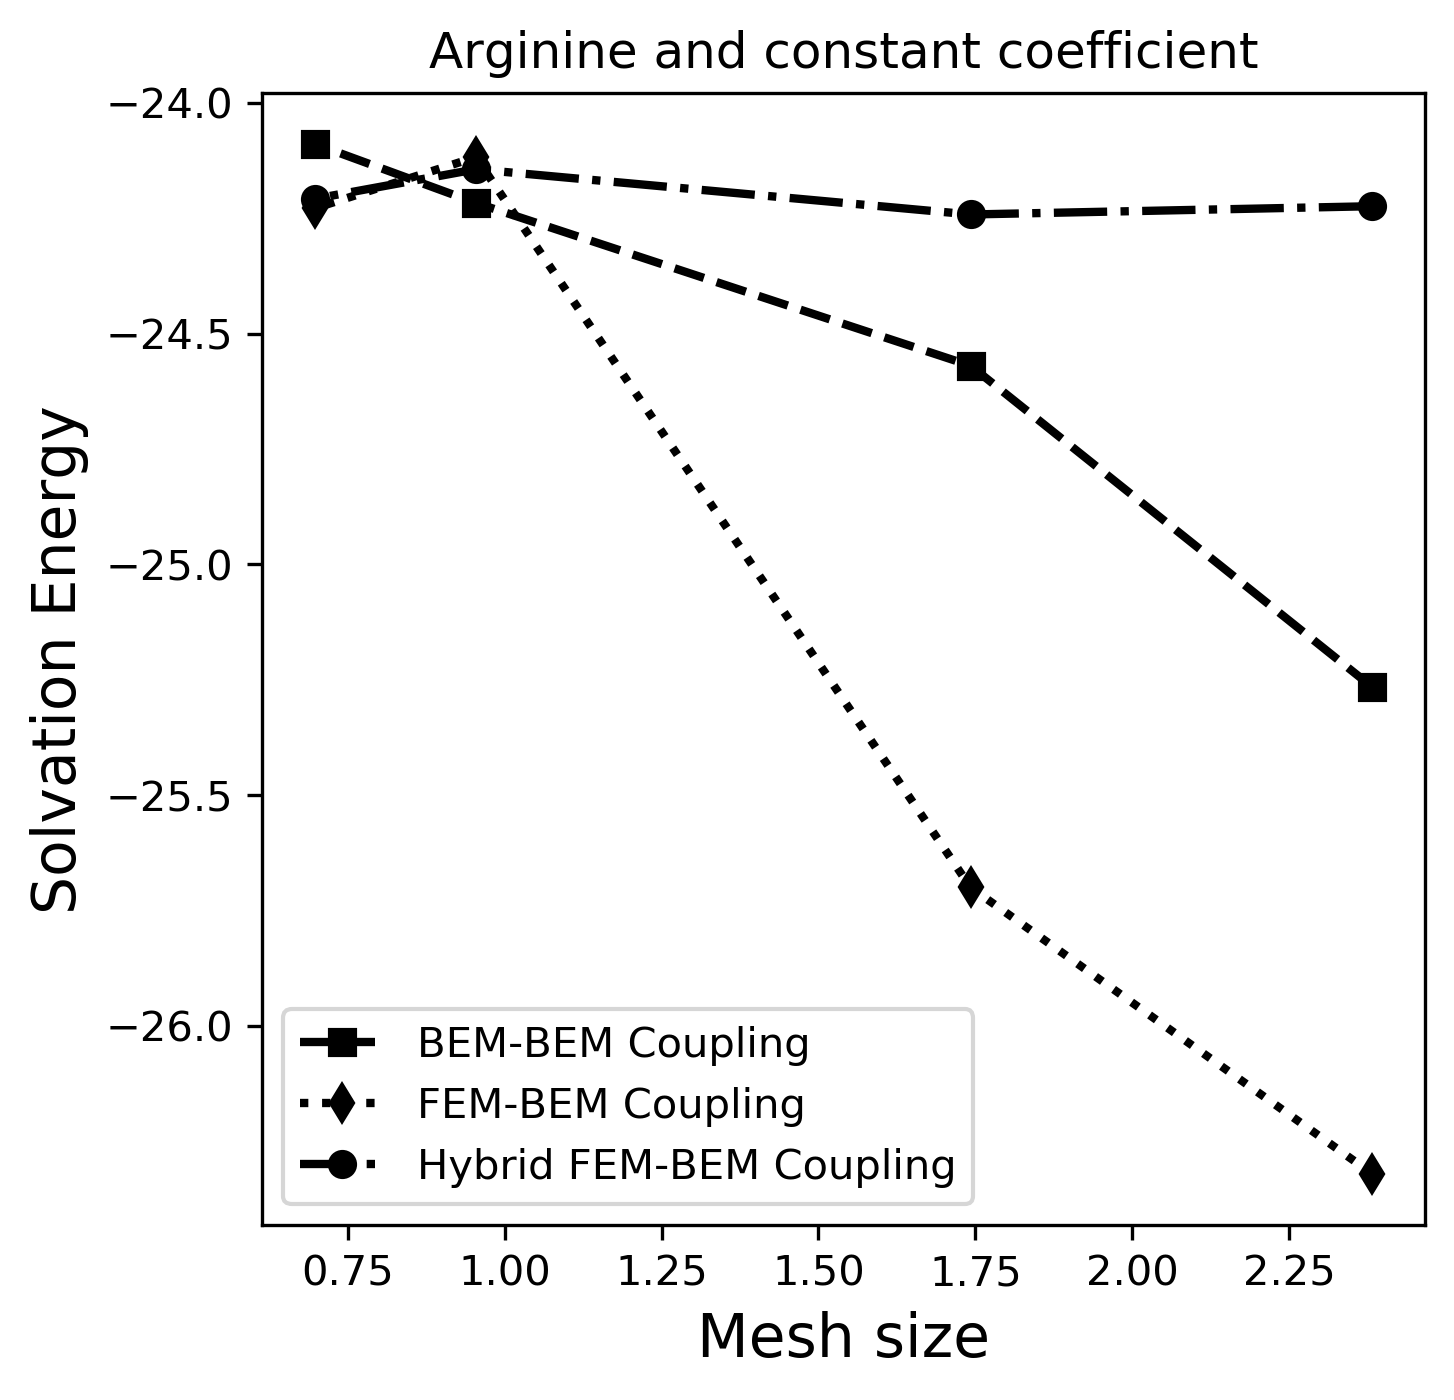
\includegraphics[width=0.45\linewidth]{Arginine_const_coeff_error.png}
%  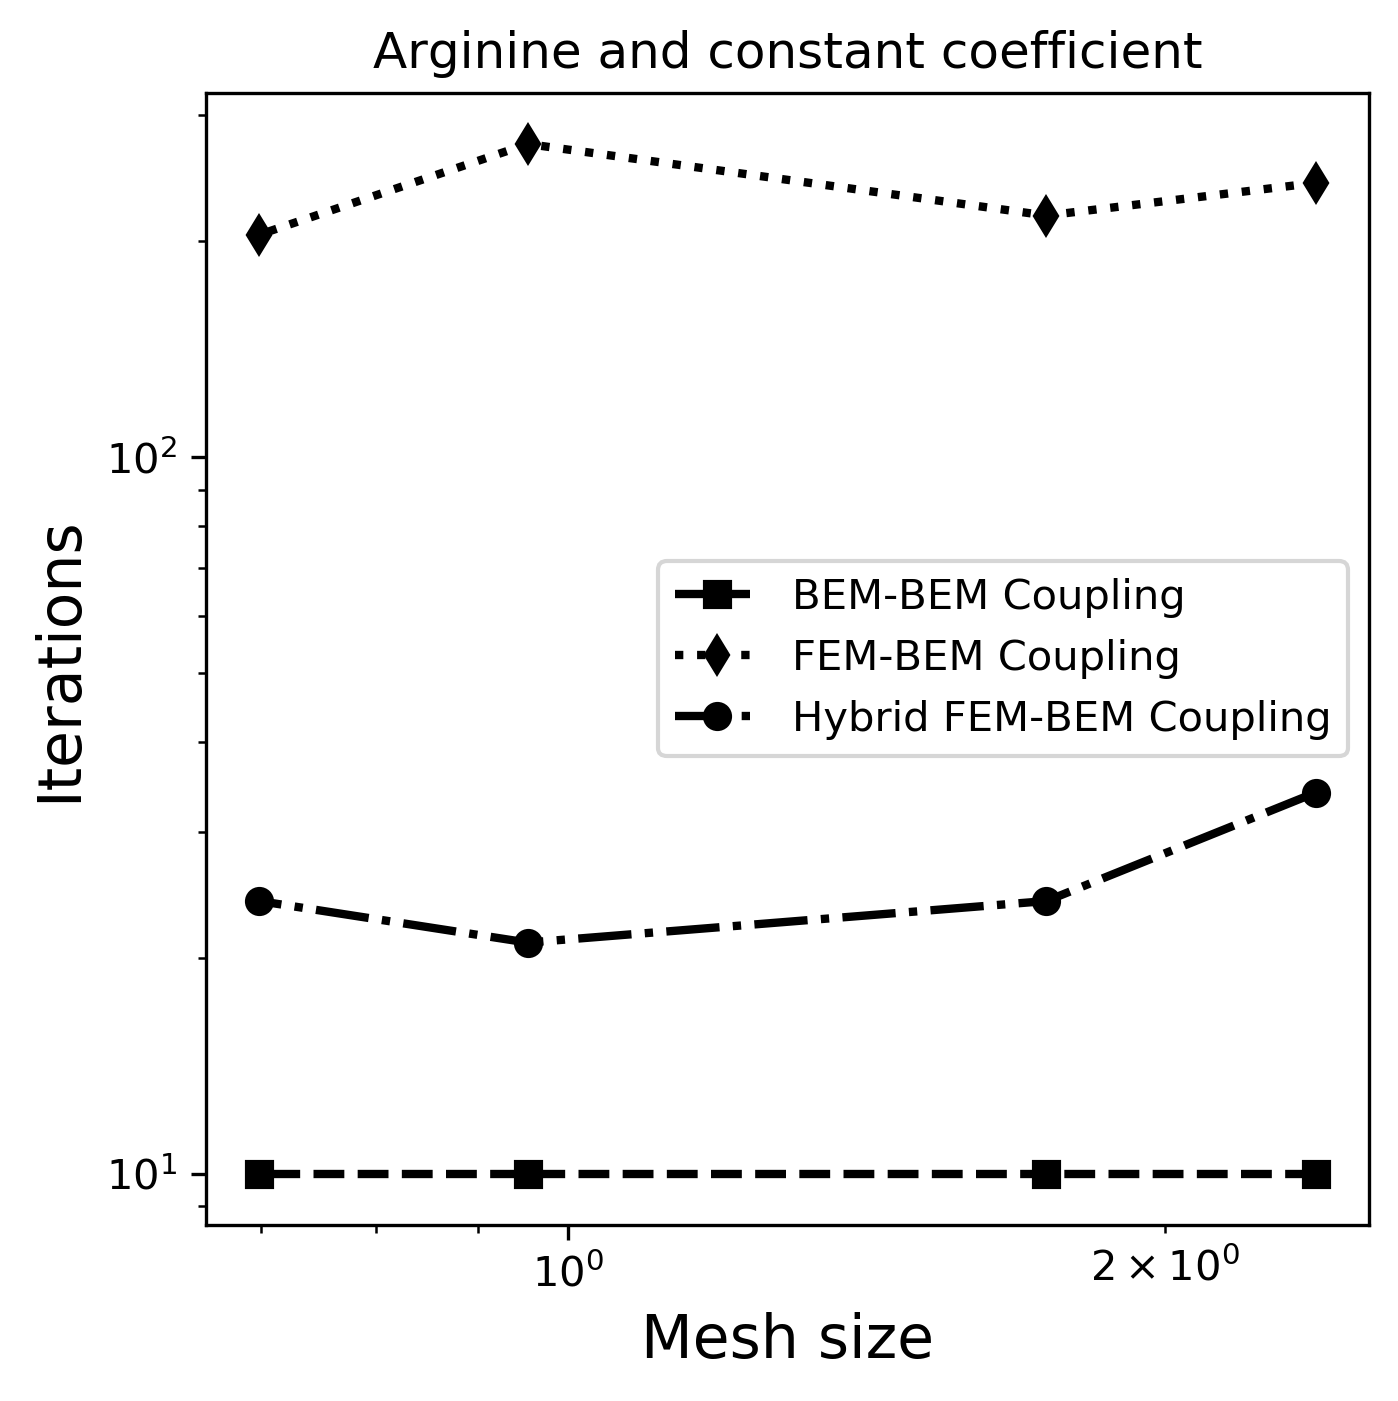
\includegraphics[width=0.45\linewidth]{Arginine_const_coeff_iter_11.png}
%%   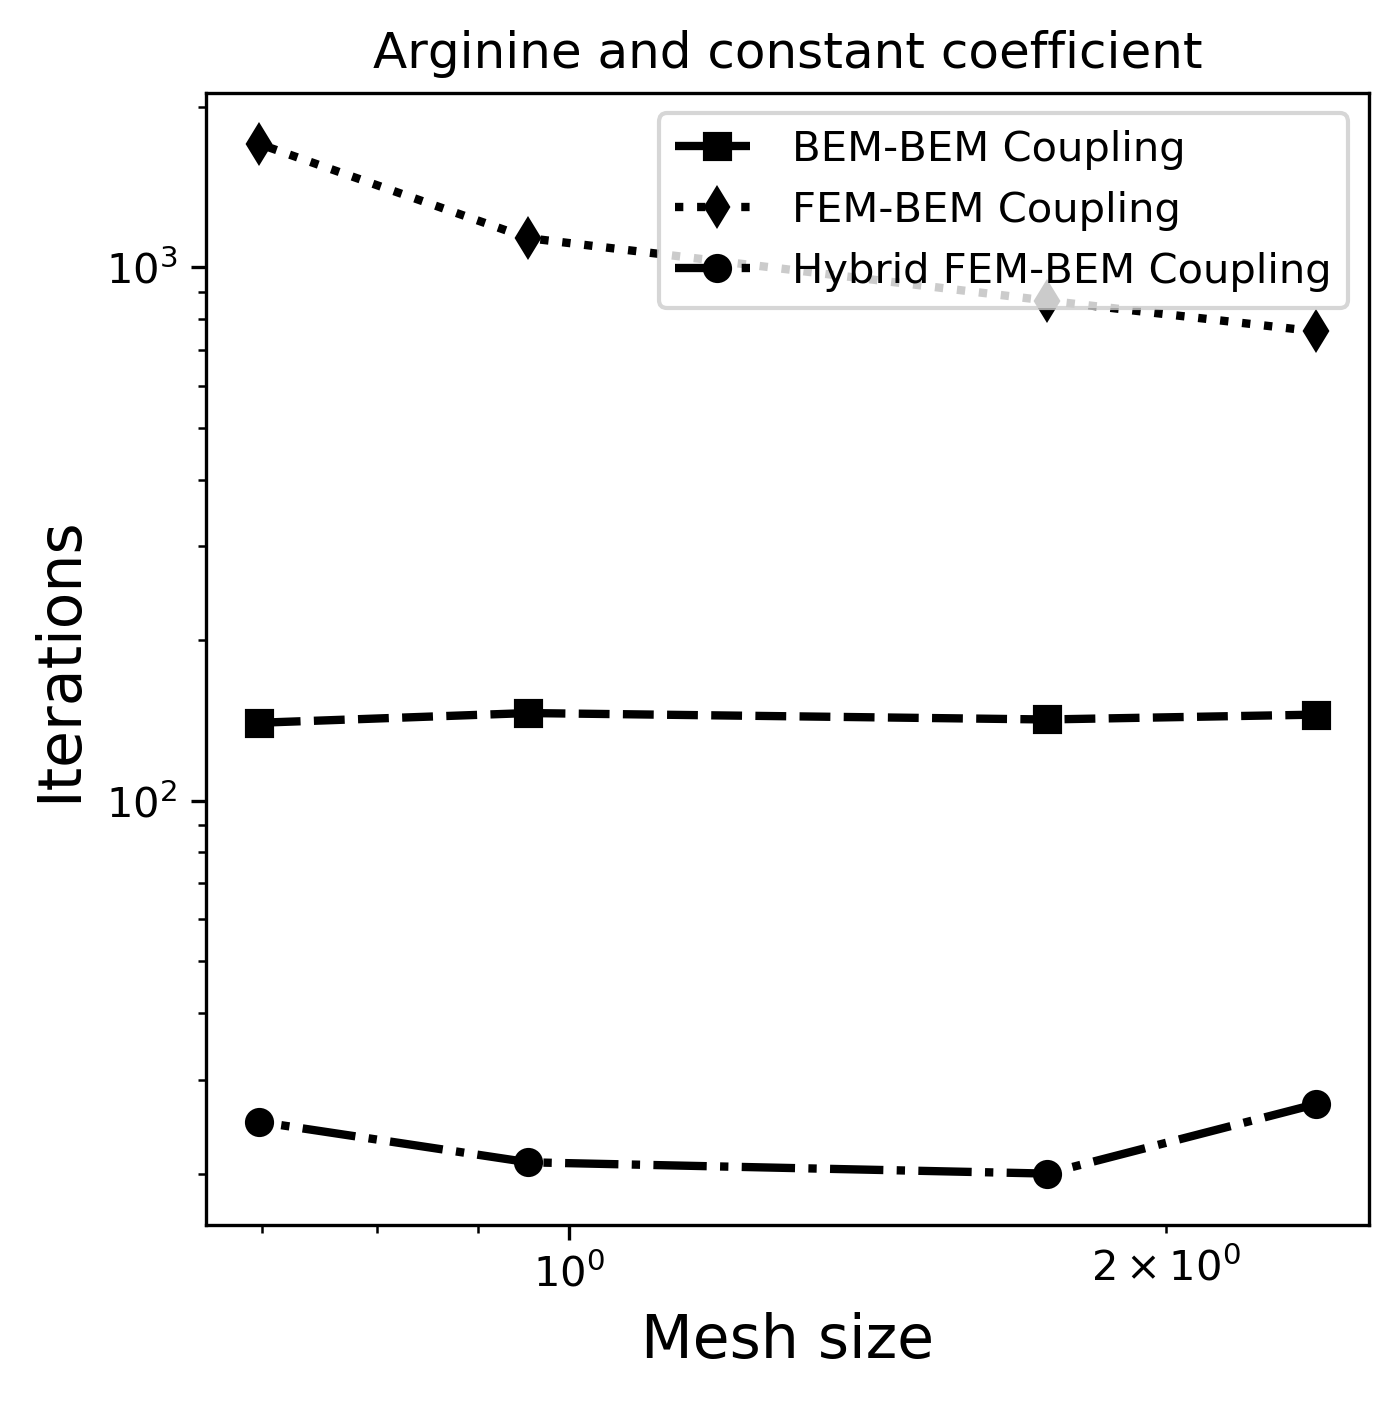
\includegraphics[width=0.45\linewidth]{No_prec_Arginine_const_coeff_iter.png}
%%   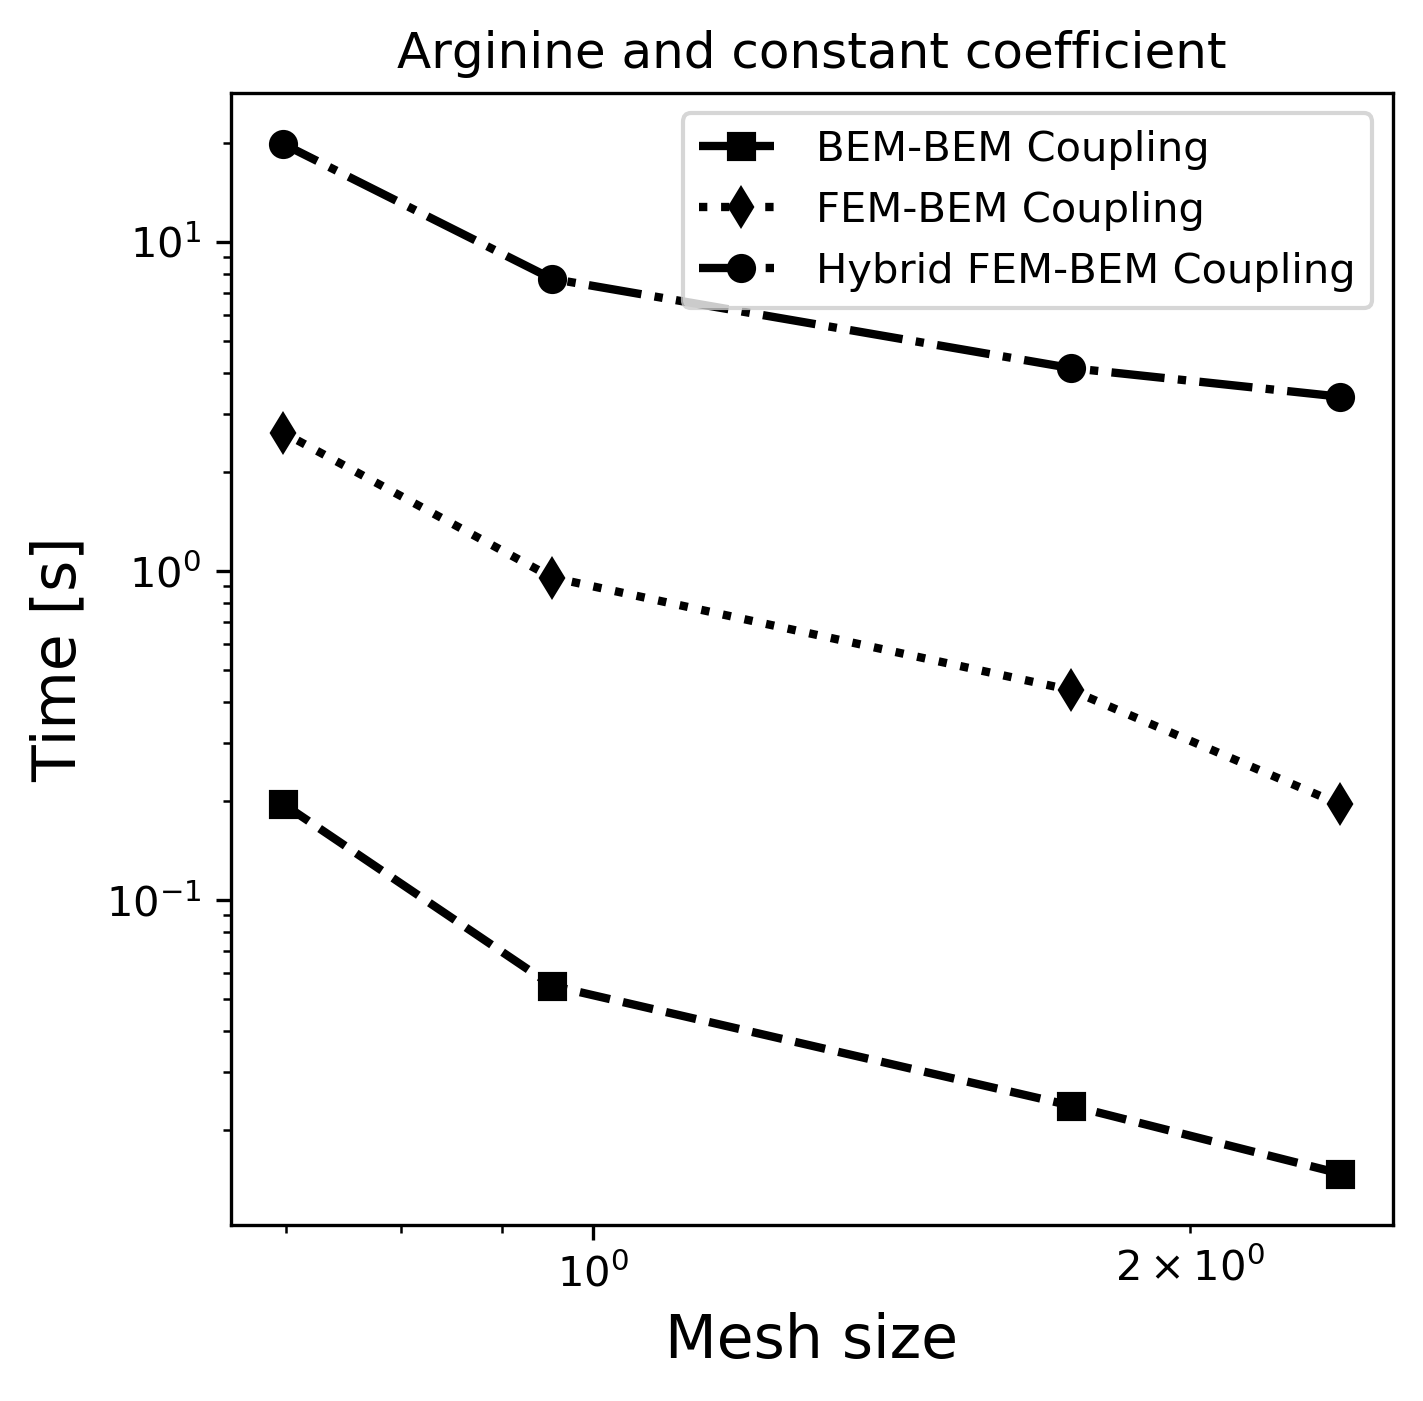
\includegraphics[width=0.45\linewidth]{Arginine_const_coeff_time.png}
%\caption{Iteration count for arginine with a constant permittivity. %(1) fix title, (2) can we put them in a single plot, (3) hybrid is internal or external iterations? maybe we should present the total count?
%}
%\label{fig:arg_contant_iter}
%\end{figure}



\section*{\sffamily \Large Results with variable permittivity}

\subsection*{\sffamily \large Motivation: modeling the solute with a Gaussian-based variable permittivity}

In contrast to a purely BEM approach, FEM-BEM coupling gives flexibility to consider space-varying field parameters. 
A popular description of the molecule is to consider a permittivity that varies like a Gaussian around each atom,\cite{grant2001smooth} which has shown enhanced accuracy in some applications, like pKa calculations.\cite{li2013dielectric}
In this setting, we define a density function $\rho$ depending on position $r$ as
%
\begin{equation}
\rho(r) := \prod_i \left(1 - \exp{\left(\frac{\|r-\mathbf{x}_i\|}{\sigma^2 R_i^2}\right)}\right)
\end{equation}
%
where the product runs over all the atoms of the solute, $R_i$ is the van der Waals radius of atom i, and we used $\sigma$=1. Then, we can compute the permittivity as
%
\begin{equation}\label{eq:varying_eps}
\epsilon := \left(1-\rho \right) \epsilon_1 + \rho\epsilon_2
\end{equation}

As $\epsilon$ is variable, Equation \eqref{eq:phic} does not have an analytical solution, and the electrostatic potential in the vacuum state has to be computed numerically.
For vacuum calculations, we considered the same distribution of $\epsilon$ inside the molecule as in the solvated case, but the solvent permittivity was set to $\epsilon_2$=2. 
Other implementations of Gaussian permittivities also modify the solute permittivity in vacuum calculations, according to a set cutoff.\cite{li2013dielectric} We did not consider a cutoff in our calculations.


We used Equation \eqref{eq:varying_eps} to generate dielectric maps, which we ran on APBS~\cite{BakerETal2001} for comparison. 
We chose APBS because it provides an easy interface to control dielectric maps, in order to ensure their agreement with the maps imposed in our FEM-BEM coupled approach.

\subsection*{\sffamily \large Convergence and performance for arginine}

Table \ref{table:arg_variable} shows a comparison of solvation energy computed with APBS and our FEM-BEM coupling approach. We can see that they are both converging to equivalent values, where the finest meshes agree up to 1.5\% {\color{red} (shouldn't be 0.5\%?)} (0.5 kcal/mol).

Figure \ref{fig:arg2_variable} contains the performance results of this test case, where we distinguish the iteration count from the calculation in dissolved and vacuum states. 

\begin{table}
\centering
\begin{tabular}{c|c|c}
&Mesh size & $\Delta G_{solv}$\\
&\AA       &  kcal/mol \\
\hline
\multirow{4}{*}{APBS}& 0.52$\times$0.52$\times$0.52 & -107.6186 \\ 
& 0.39$\times$0.39$\times$0.39 & -107.8752\\ 
&0.26$\times$0.26$\times$0.26 & -108.3378\\ 
&0.195$\times$0.195$\times$0.195 & -108.5837\\ 
&0.098$\times$0.098$\times$0.098 & -108.8844\\ 
\hline
&Mesh dens. & \\
&vert/\AA$^2$ & \\
\hline
%\multirow{5}{*}{Standard FEM-BEM}& 2 & -36.239\\
    & 4.1 & -109.933 \\
FEM-BEM    & 6.7  & -110.238 \\
coupling    & 8.57  & -109.658 \\
    & 17 & -109.368 \\
    & 24.5 & -109.286 \\
\hline
%\multirow{5}{*}{Standard FEM-BEM}& 2 & -29.554\\
%    & 2 & -34.670\\
%Hybrid    & 4  & -33.603 \\
%FEM-BEM    & 8  & -32.822 \\
%    & 16 & -32.072 \\
%\hline
\end{tabular}
\caption{Solvation energy of arginine with a Gaussian-like permittivity, computed using the FEM-BEM approach and APBS. The mesh density for FEM-BEM corresponds to the vertex density of the surface mesh used to generate the volumetric mesh. Add performance result?}
\label{table:arg2_variable}
\end{table}

%\begin{figure}
%\centering
%% 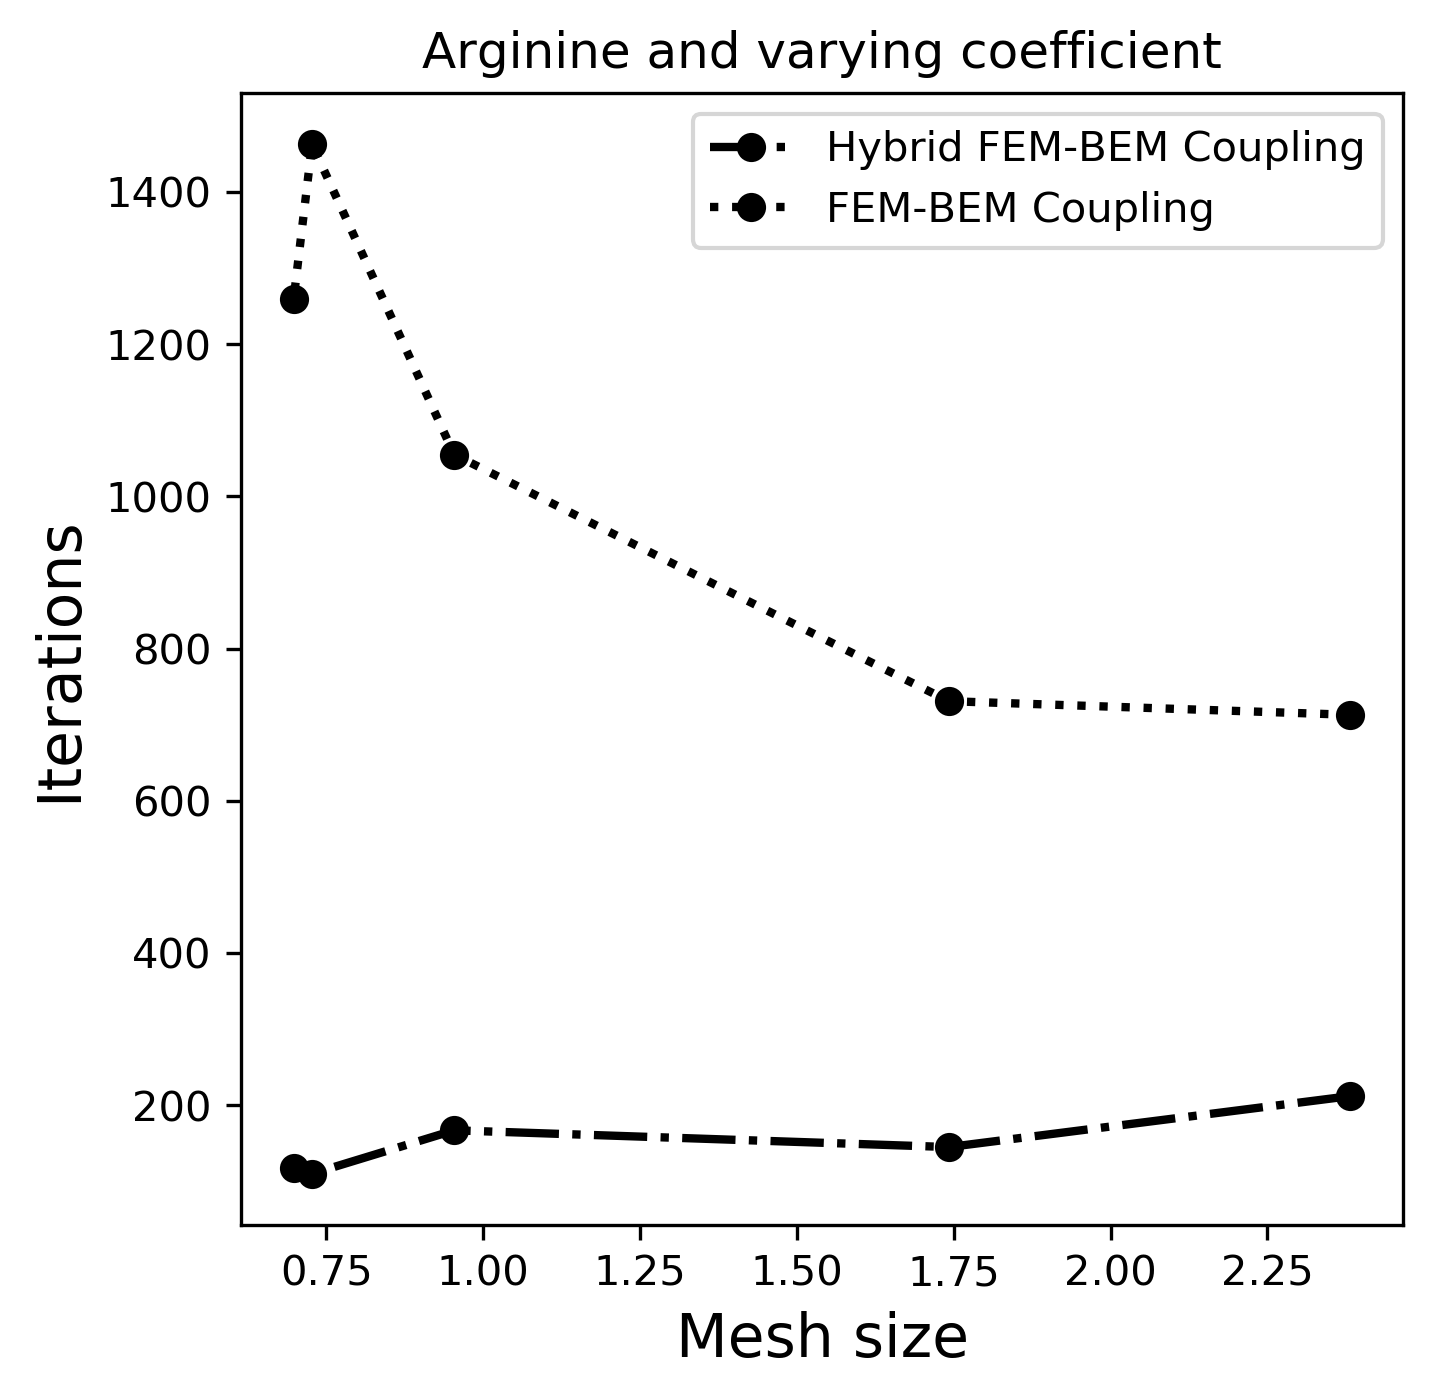
\includegraphics[width=0.45\linewidth]{Arginine_varying_coeff_iter.png}
%% 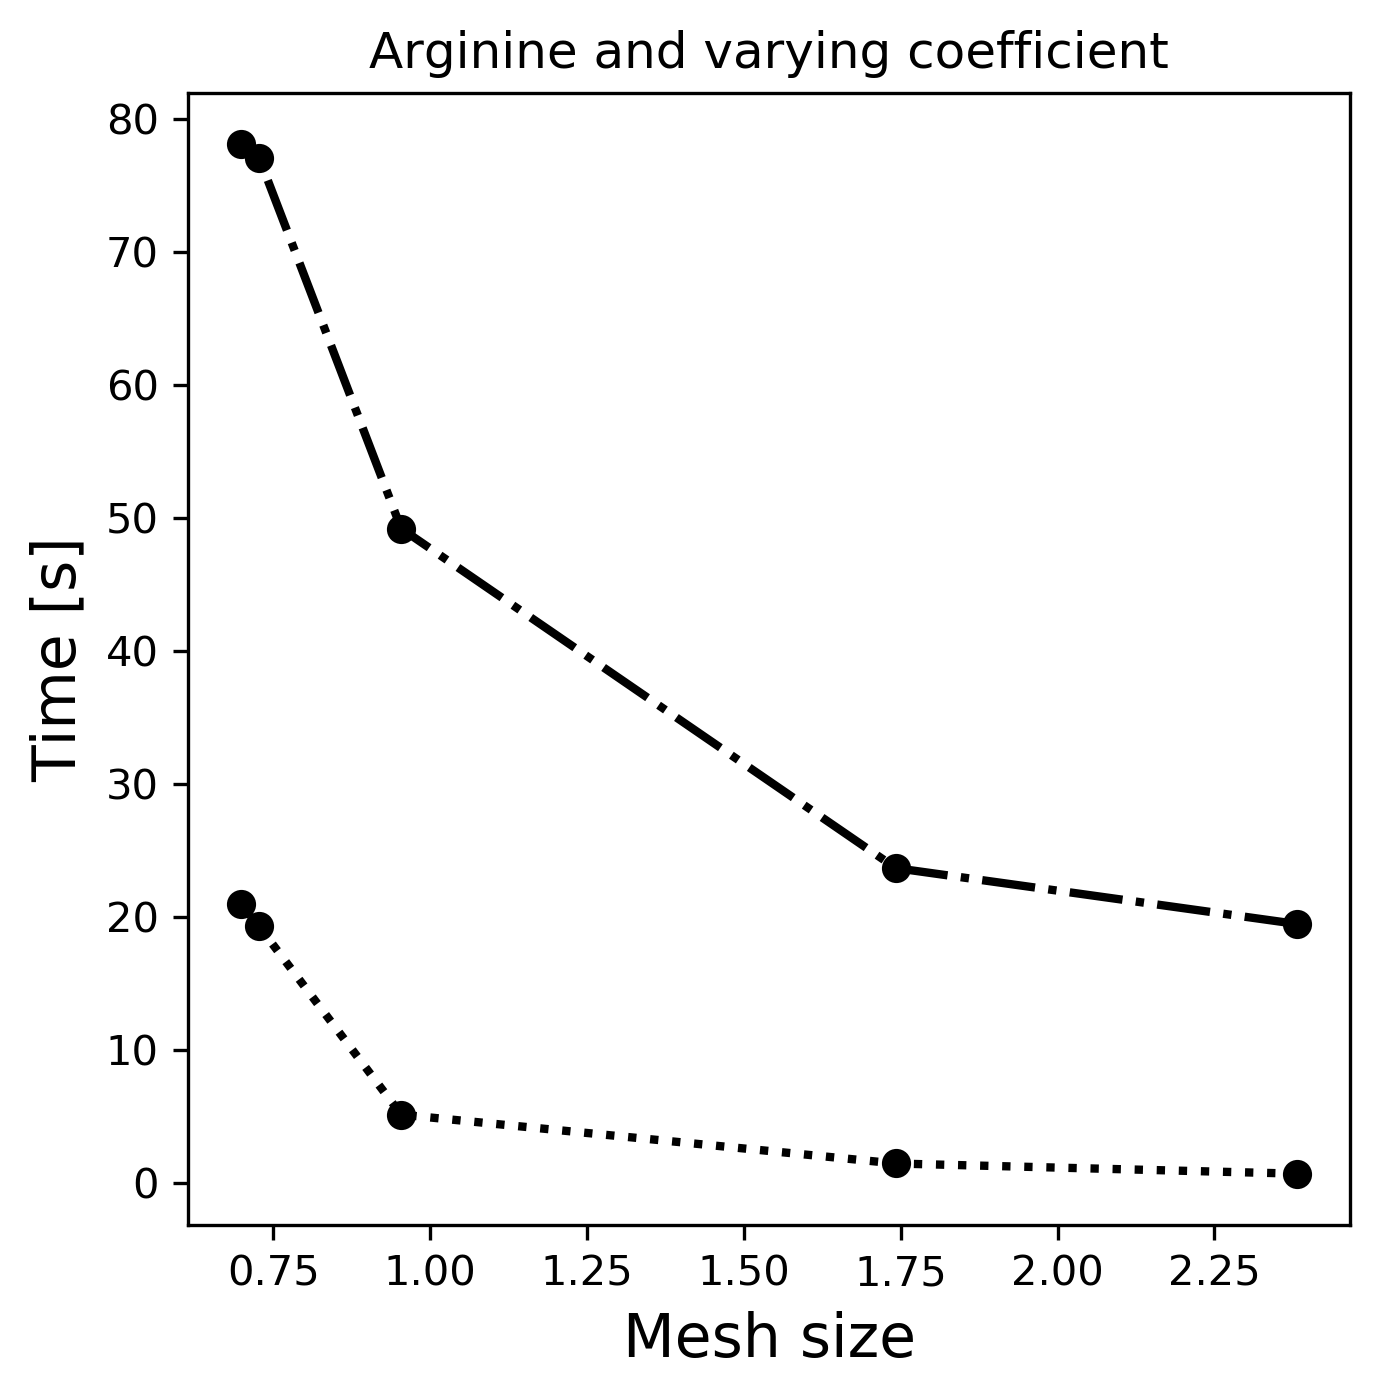
\includegraphics[width=0.45\linewidth]{Arginine_varying_coeff_time.png}
%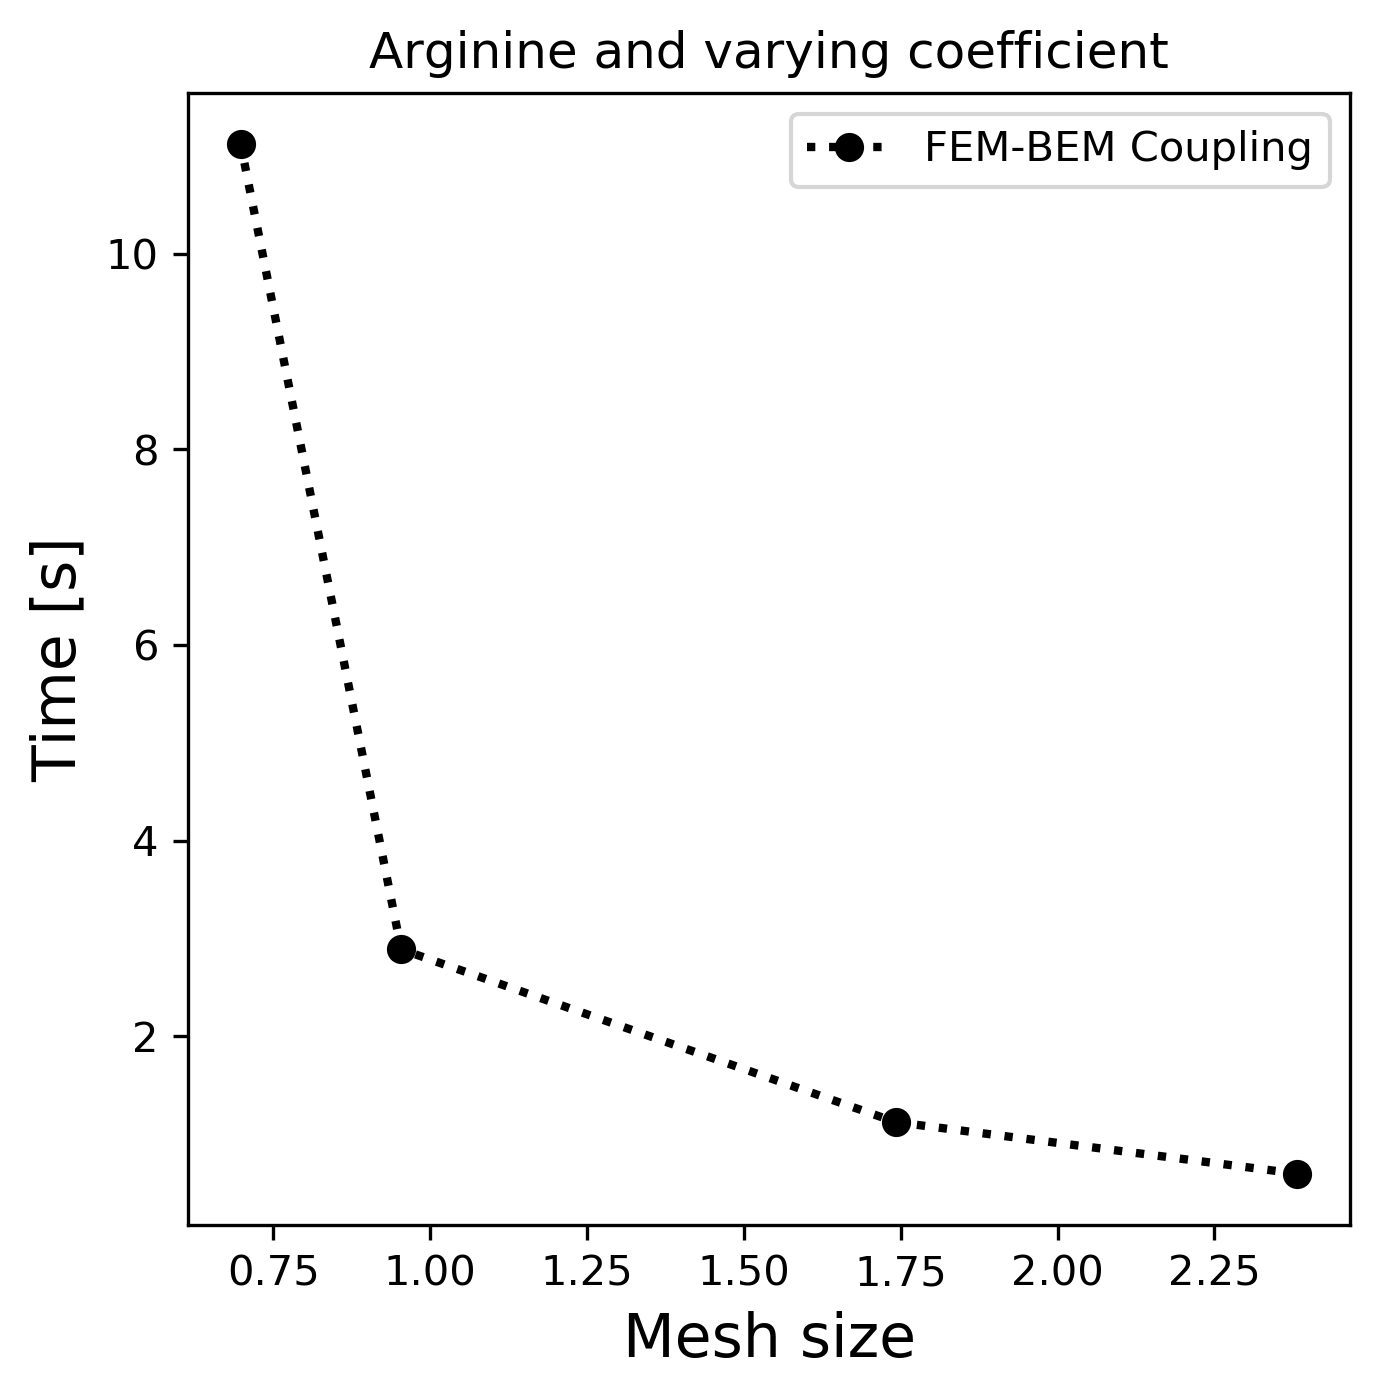
\includegraphics[width=0.45\linewidth]{Arginine_varying_coeff_time_11.png}
%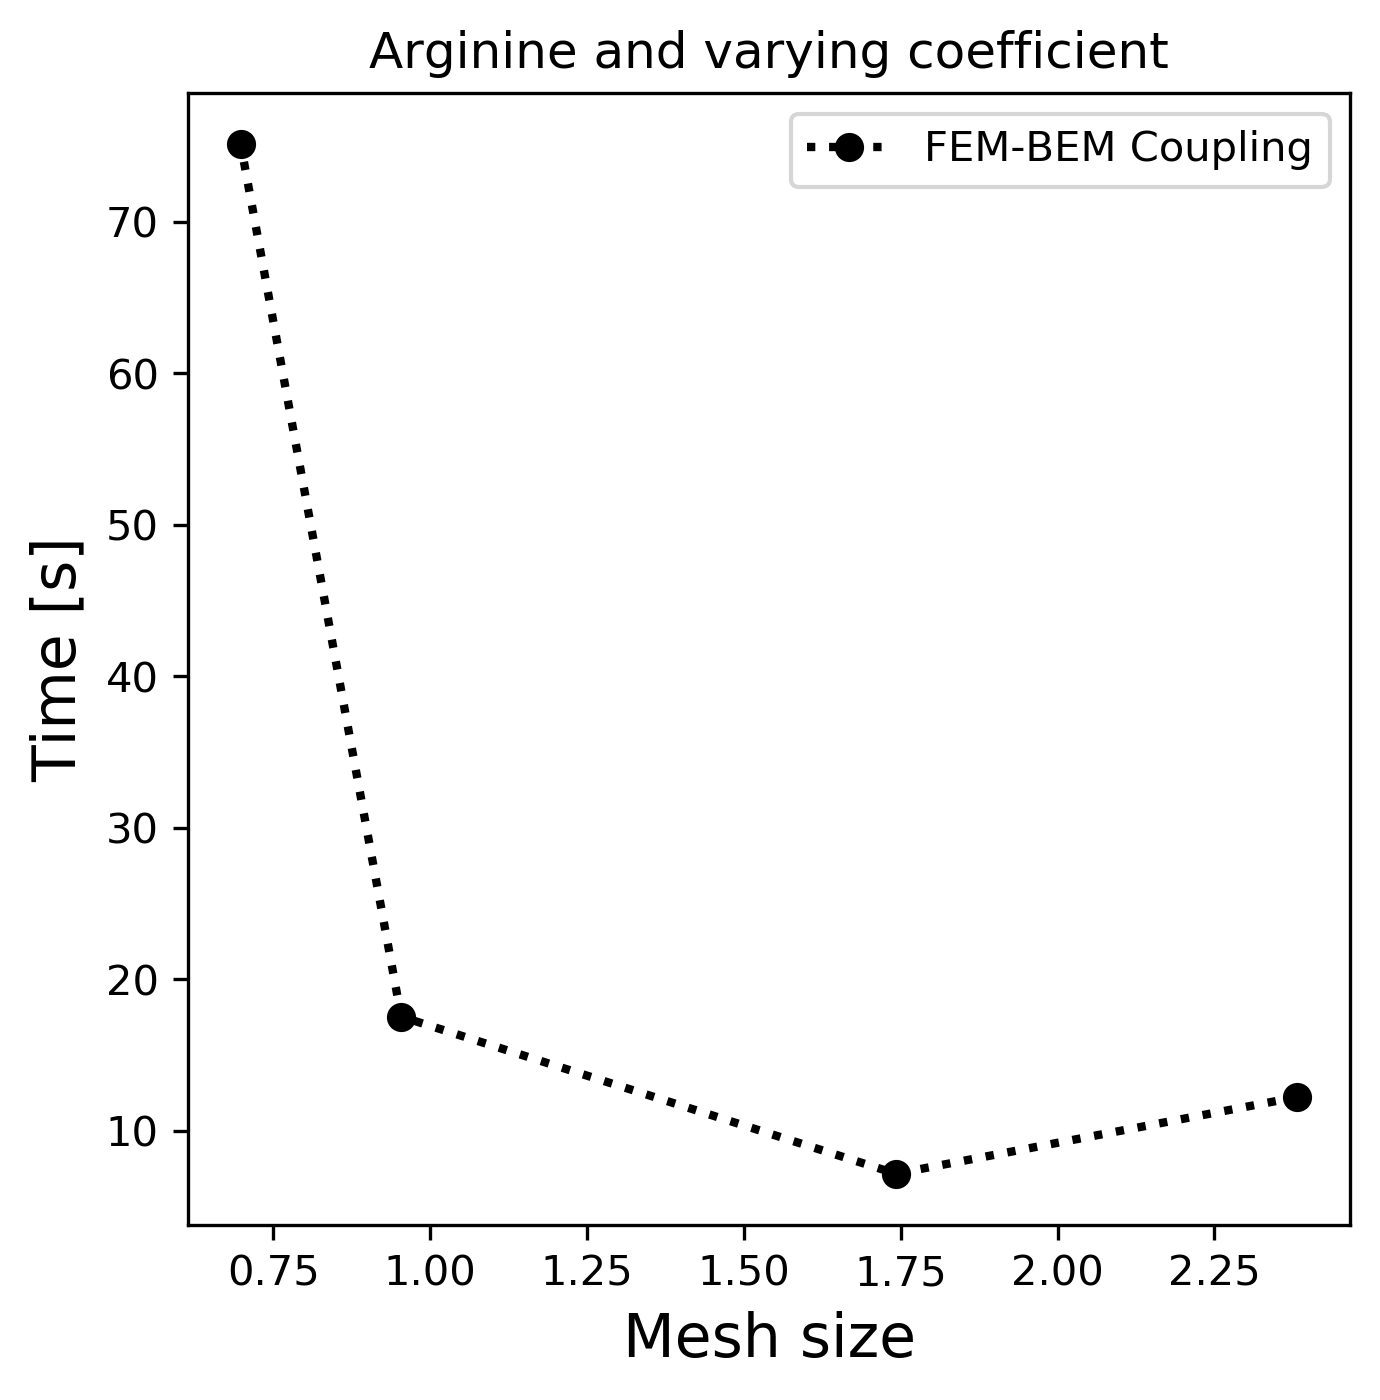
\includegraphics[width=0.45\linewidth]{Arginine_varying_coeff_setup_time_11.png}
%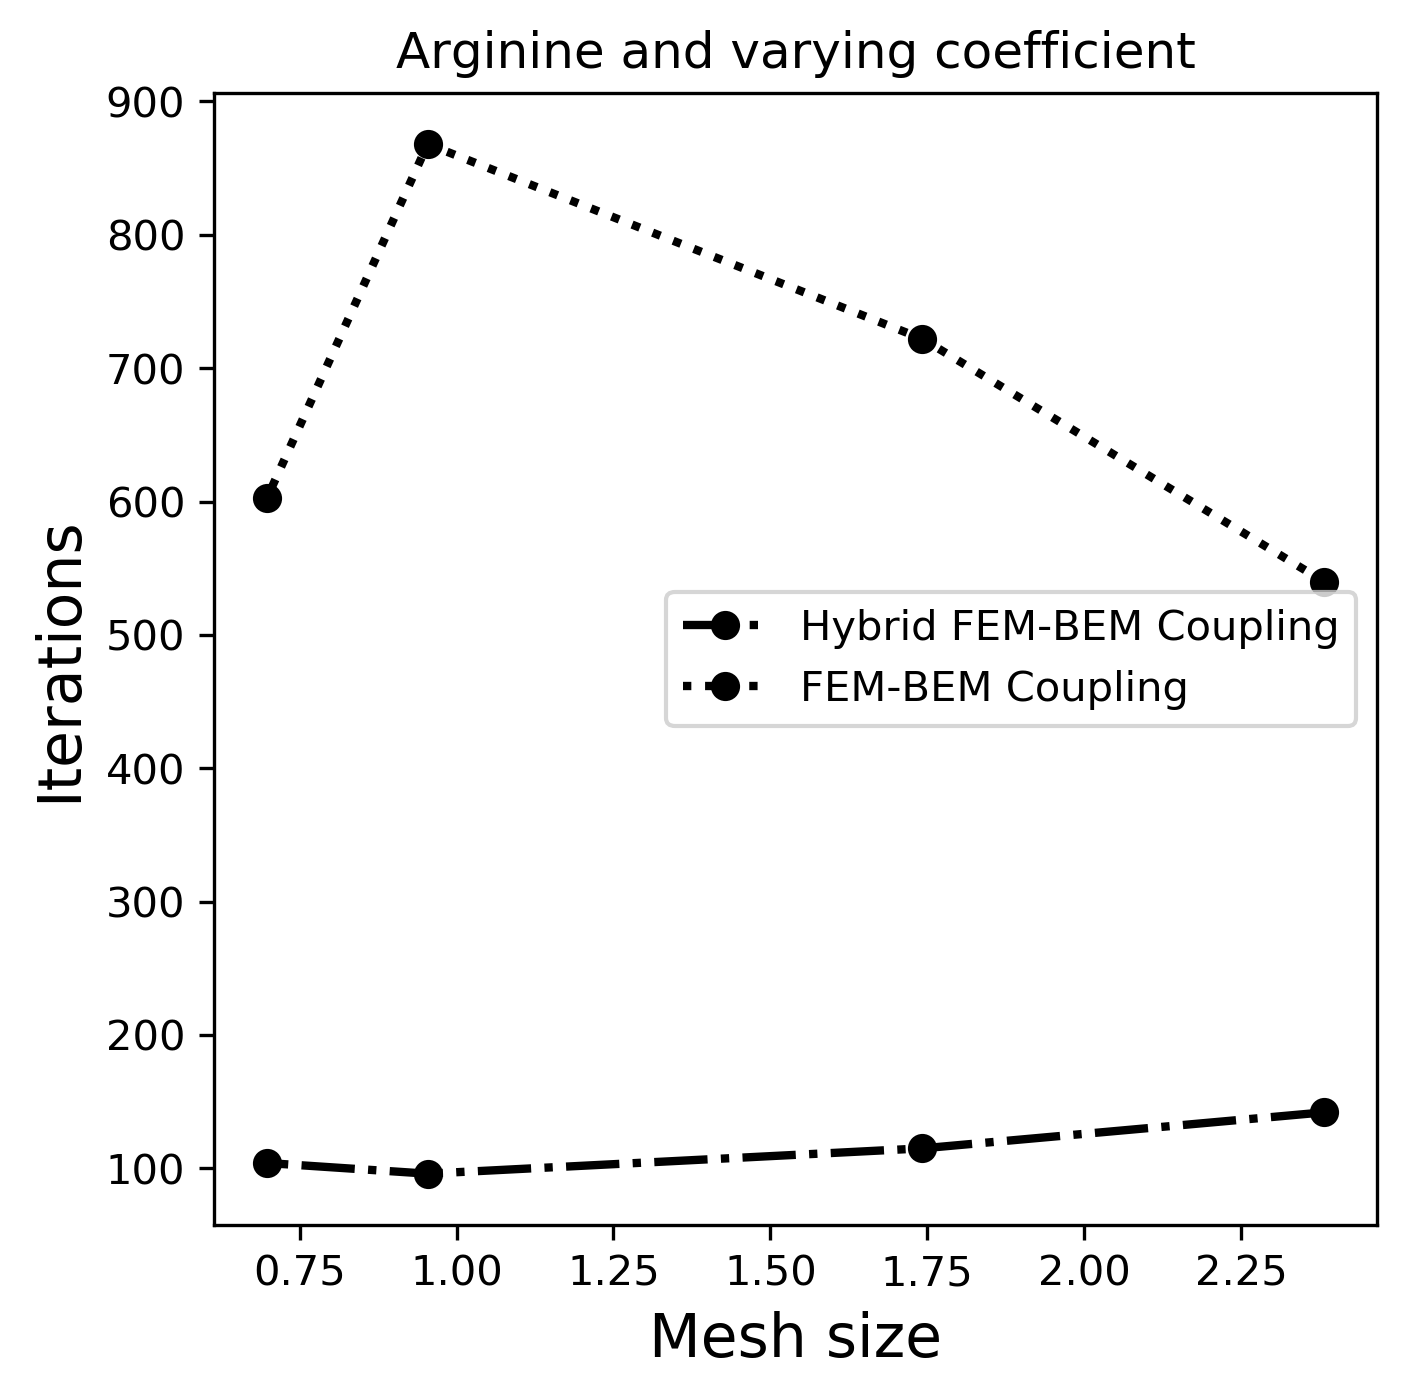
\includegraphics[width=0.45\linewidth]{Arginine_varying_coeff_iter_11.png}
%\caption{Iteration count and time-to-solution to compute the solvation energy of arginine with a variable permittivity (left: Online time taken to solve systems, right: Offline time taken to set up systems), using FEM-BEM coupling. %Can we make this only two plots?
%}
%\label{fig:arg_variable}
%\end{figure}

\begin{figure}
\centering
% 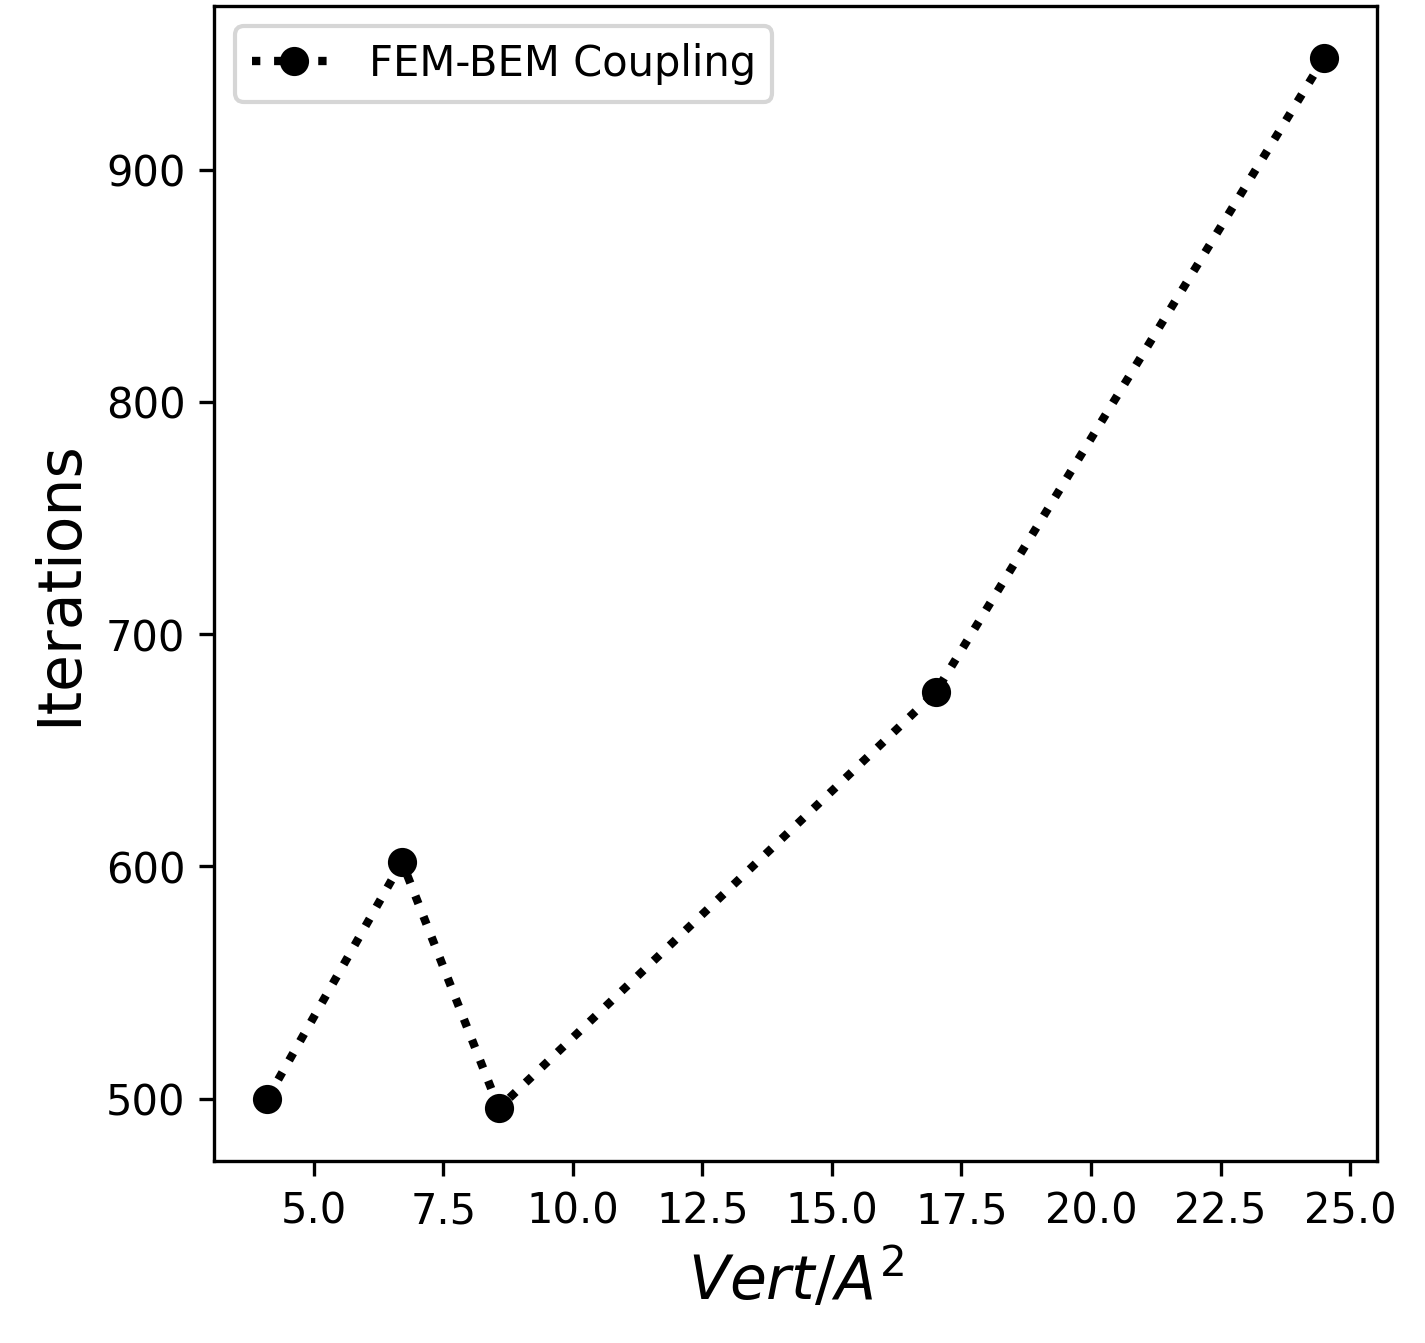
\includegraphics[width=0.45\linewidth]{DolfinX_Arginine2_varying_coeff_iter.png}
% 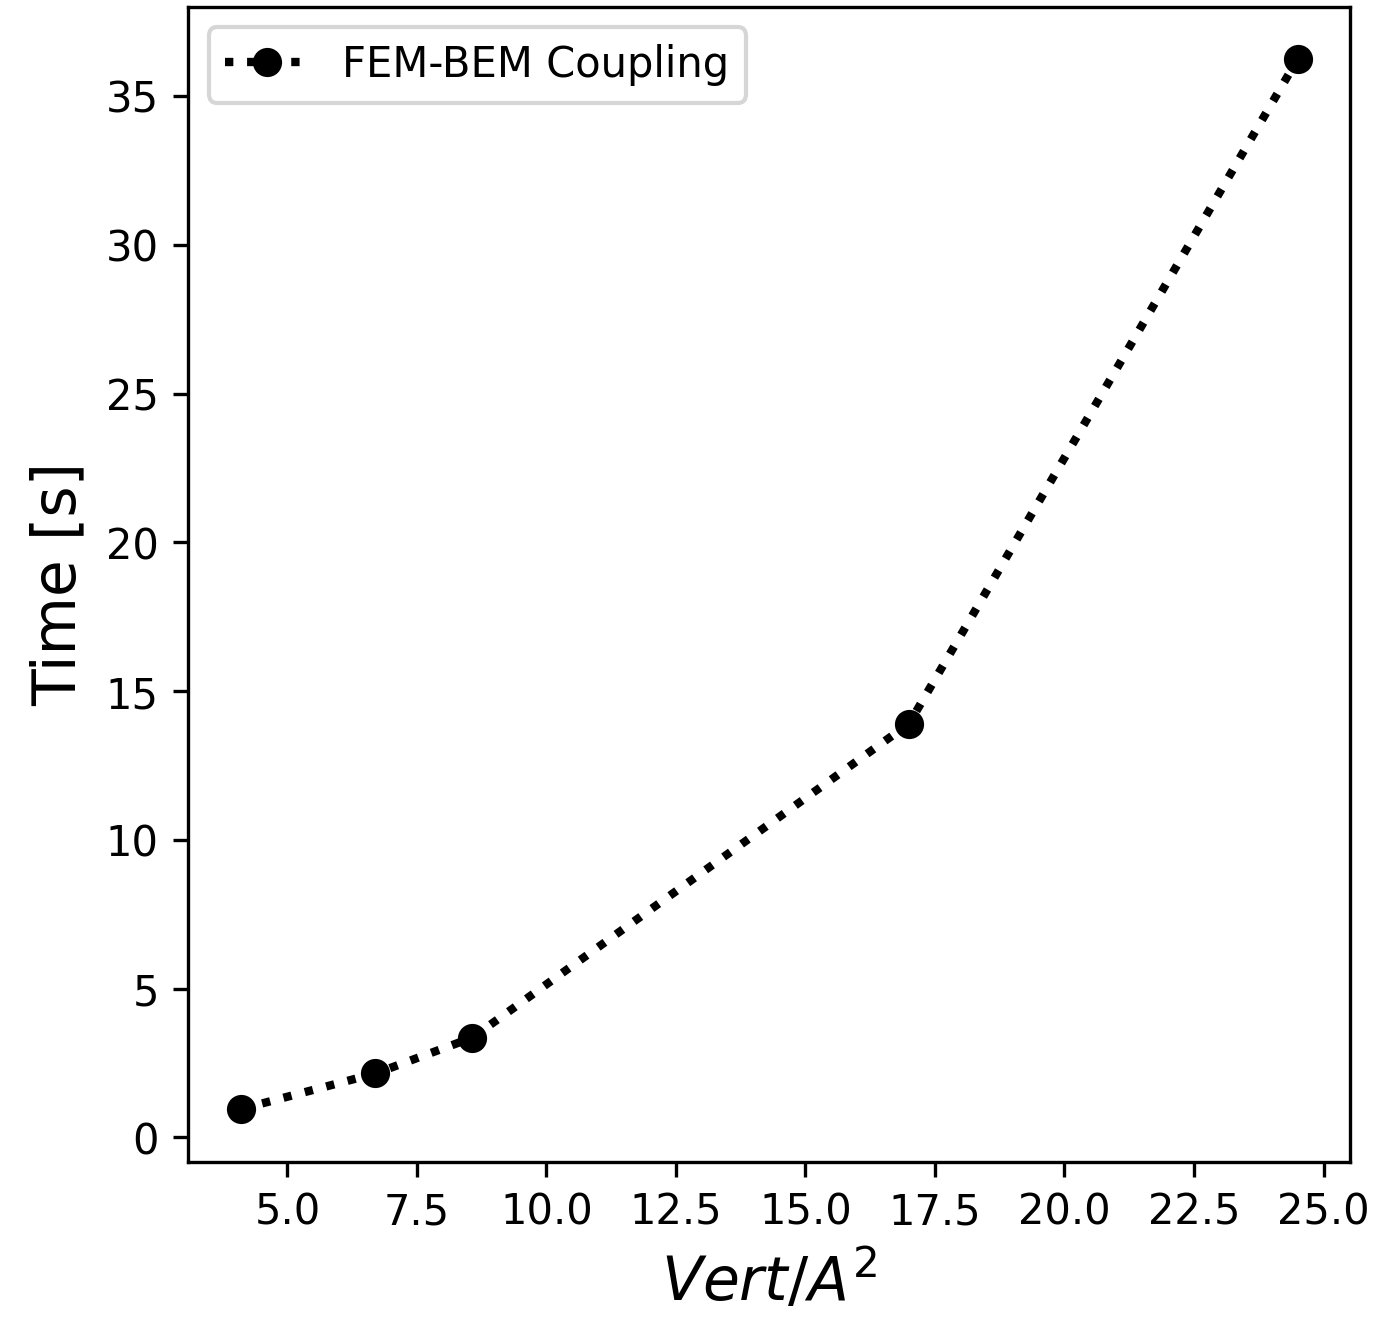
\includegraphics[width=0.45\linewidth]{DolfinX_Arginine2_varying_coeff_time.png}
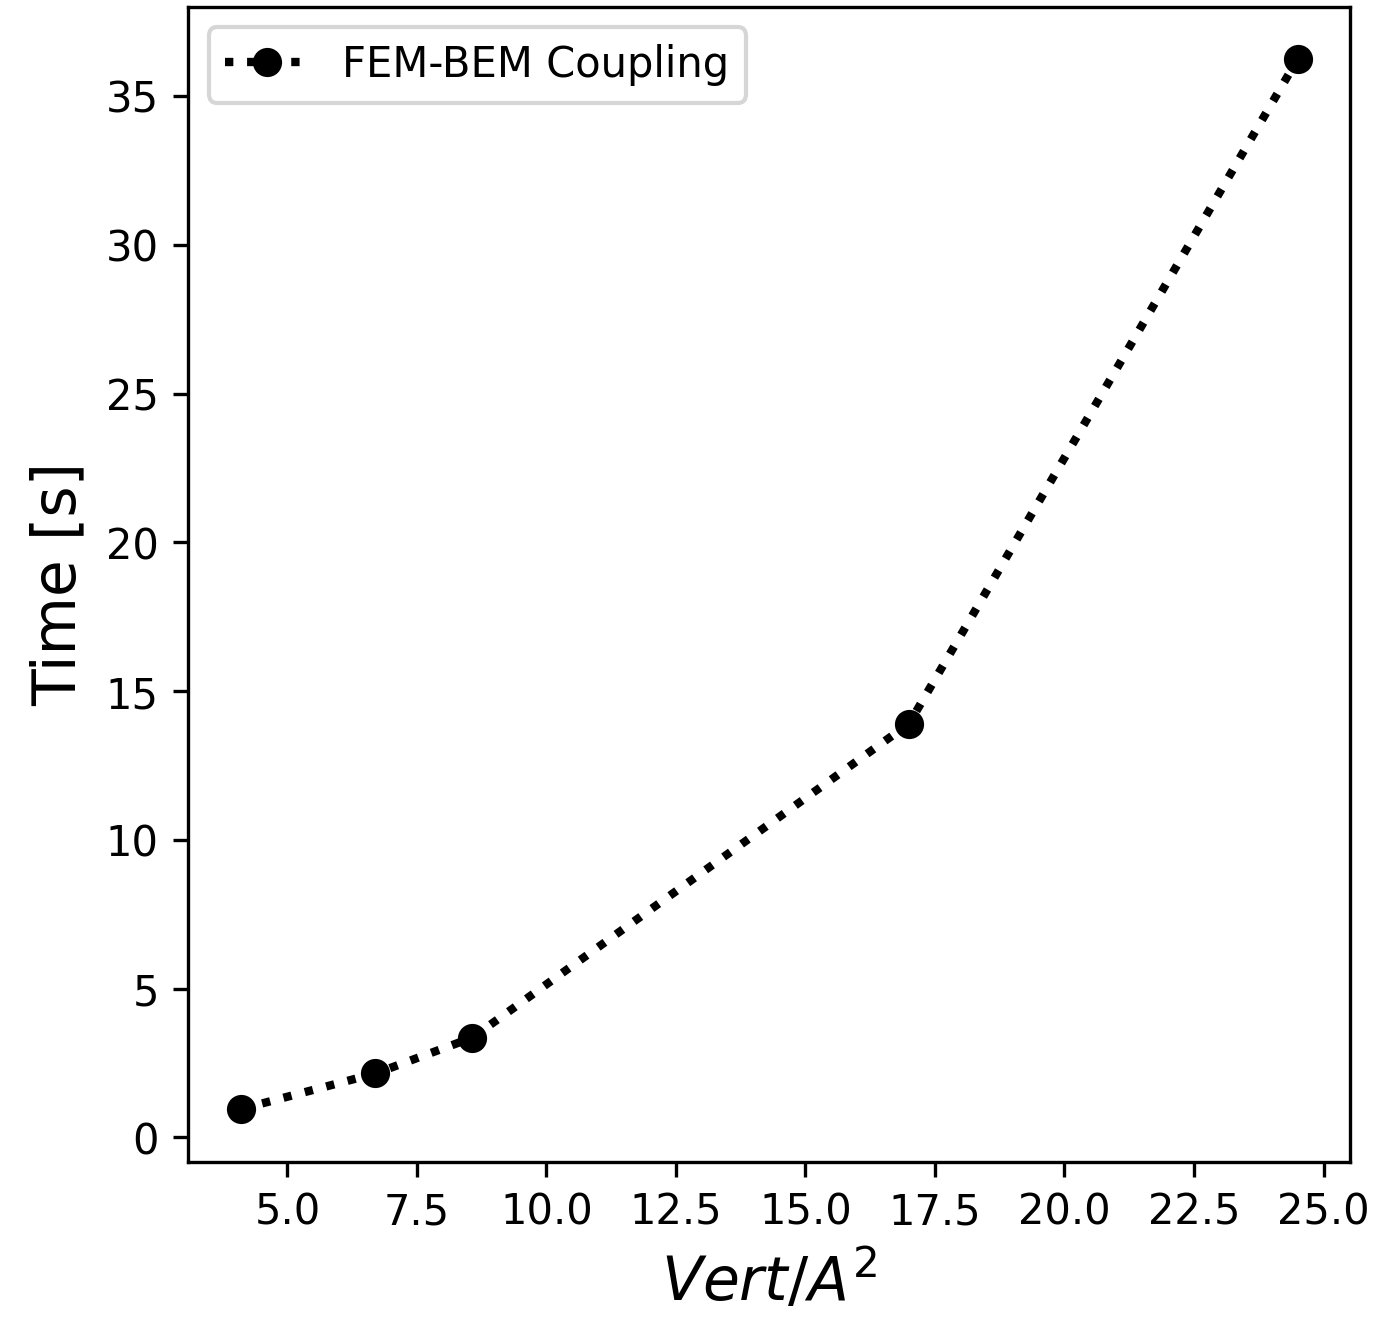
\includegraphics[width=0.45\linewidth]{DolfinX_Arginine2_varying_coeff_time.png}
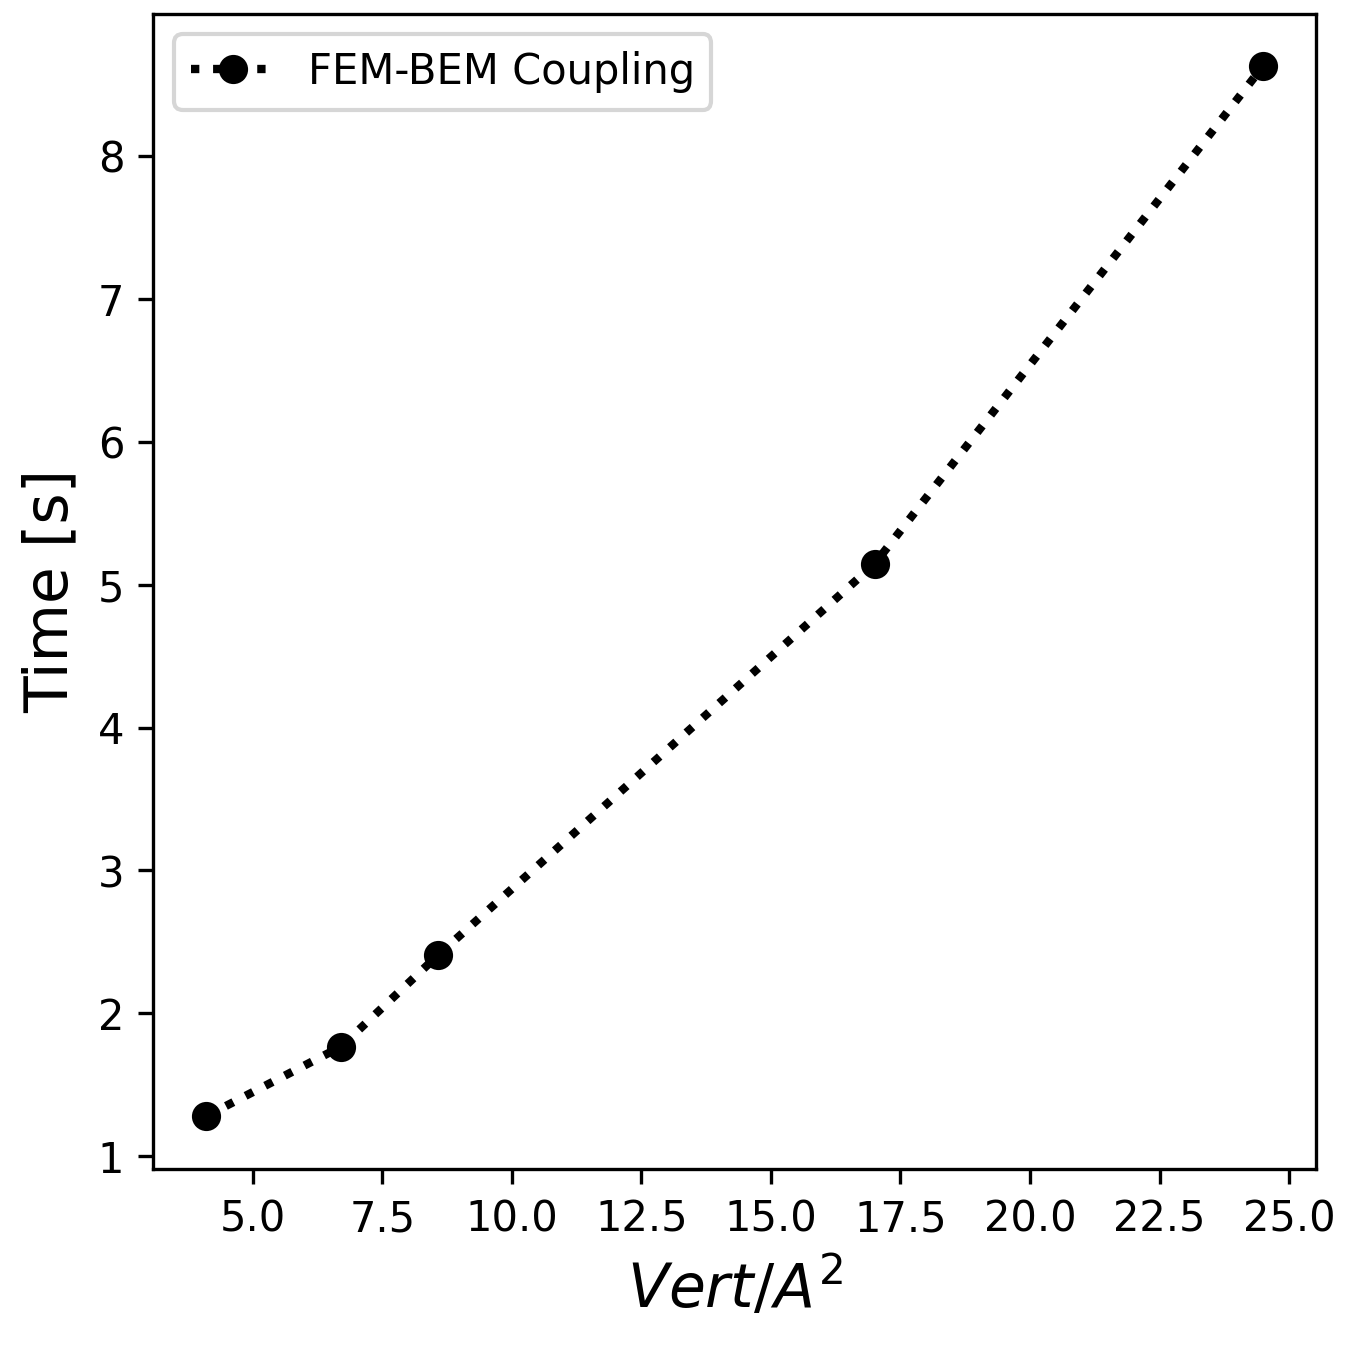
\includegraphics[width=0.45\linewidth]{DolfinX_Arginine2_varying_coeff_set_time.png}
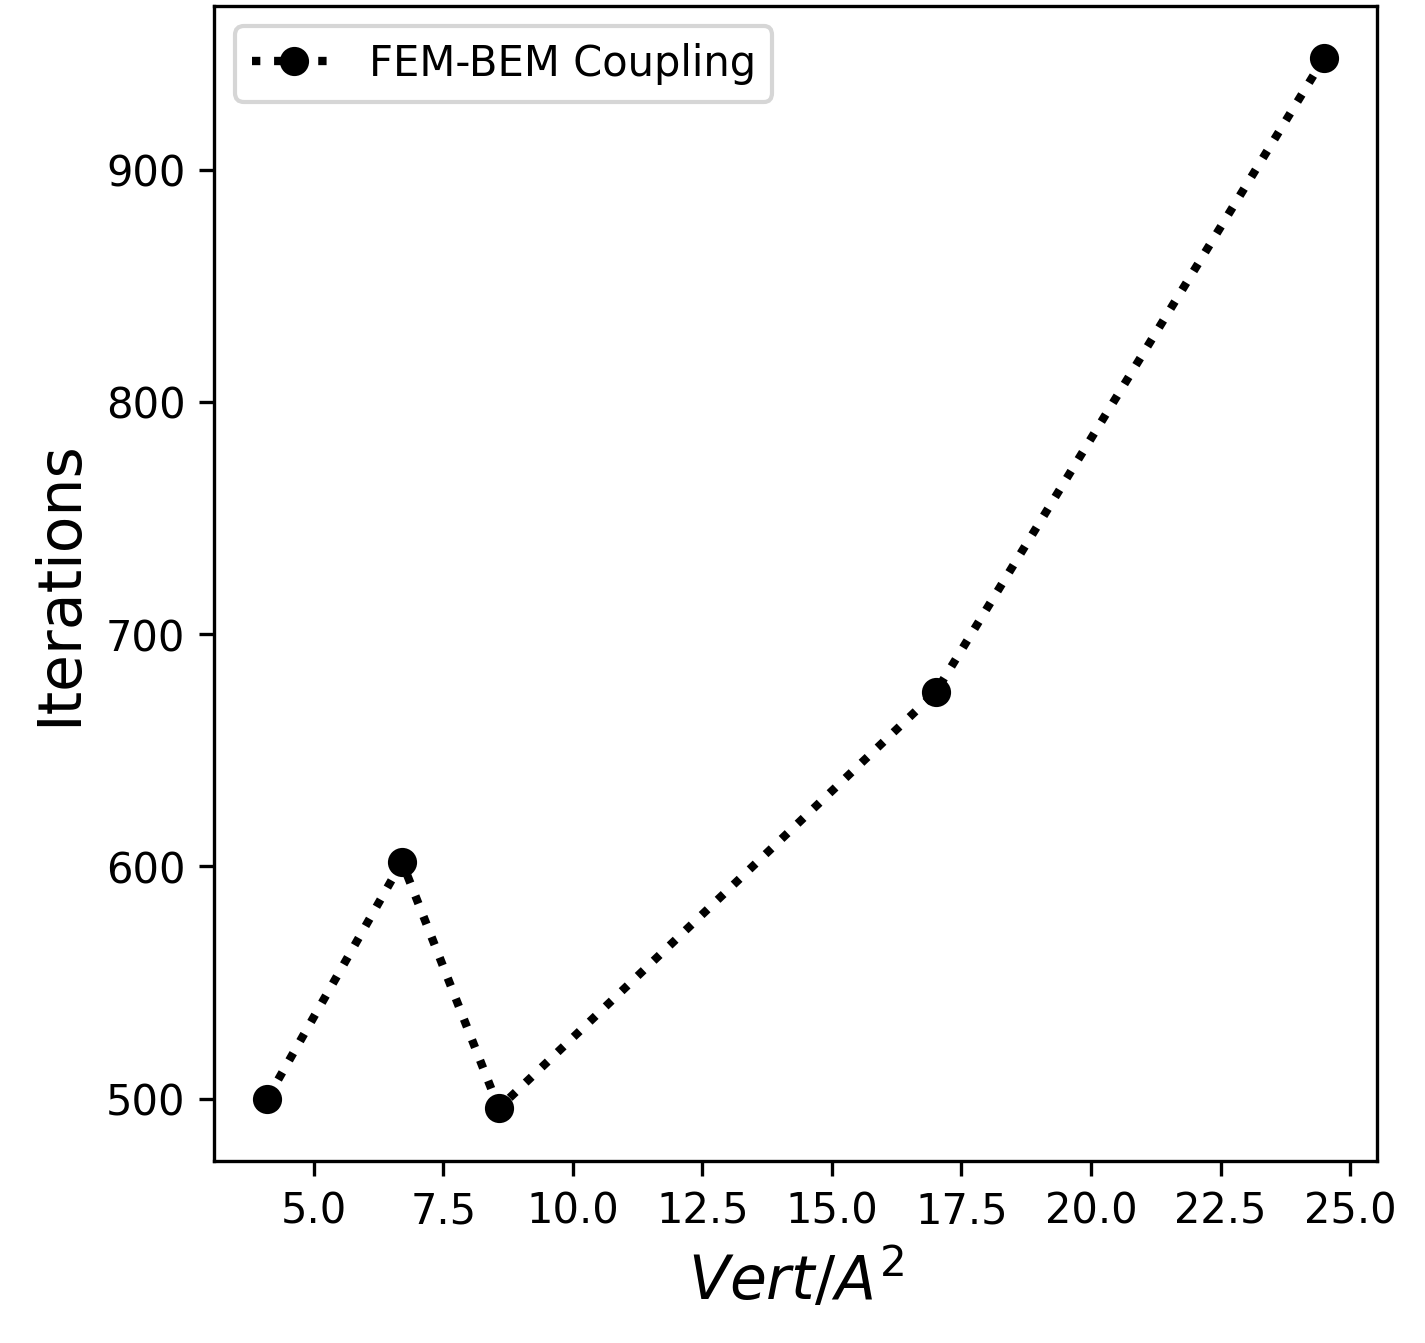
\includegraphics[width=0.45\linewidth]{DolfinX_Arginine2_varying_coeff_iter.png}
\caption{Iteration count and time-to-solution to compute the solvation energy of arginine with a variable permittivity (left: Online time taken to solve systems, right: Offline time taken to set up systems), using FEM-BEM coupling. %Can we make this only two plots?
}
\label{fig:arg2_variable}
\end{figure}


\subsection*{\sffamily \large Performance analysis for larger structures}

So far, we have only tested the FEM-BEM coupled approach with small structures. Here, we study its behaviour with larger structures to evaluate its applicability in more realistic settings.


\begin{table}
\centering
\begin{tabular}{c|c|c|c|c|c|c}
Molecule & Mesh size  & $\Delta G_{solv}$ & Iterations & Setup Time & Solving Time & Total Time \\
& vert/\AA$^2$ &  kcal/mol & & sec & sec & sec \\
\hline
 1pgb &  & -300.888 & 826 & 82 & 547 & 629  \\
 1lyz &  & -599.642 & 1 285 & 330 & 1 640  & 1 970  \\
 1lyz gs3 & & -600.637 & 2 949  & 1 690 & 10 900 & 12 590   \\
 1uxu &  & -1 984.468 & 4 167 & 8 240 & 16 300 & 24 540  \\
 1igt &  &  -3 294.230 & 8 361 & 41 200 & 64 200 &  105 400   \\
 \hline
\end{tabular}
\caption{Large tests' results}
\label{table:large_variable}
\end{table}
